\documentclass[../DoAn.tex]{subfiles}
\begin{document}

\section{Thiết kế kiến trúc}
\subsection{Lựa chọn kiến trúc phần mềm}
Website đấu giá trực tuyến được xây dựng dựa theo mô hình MVC. Sau đây em xin trình bày tổng quát về mô hình MVC thông qua hình vẽ bên dưới: 
\begin{figure}[H]
    \centering
    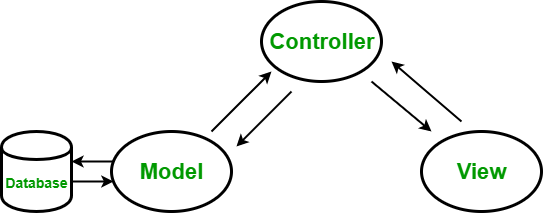
\includegraphics[width=10.6cm,height=4.15cm]{Hinhve/mvc.png}\cite{MVC}
    \caption{Mô hình kiến trúc MVC}
    \label{fig:Fig41}
\end{figure}
Mô hình MVC là mẫu kiến trúc phân chia ứng dụng thành 3 thành phần chính: Model, View, Controller. Mỗi thành phần được xây dựng để xử lý các tác vụ khác nhau của một ứng dụng\cite{MVC2}.
\begin{itemize}
    \item Lớp dữ liệu (Model) chịu trách nhiệm quản lý dữ liệu của ứng dụng, tương tác với hệ quản trị cơ sở dữ liệu. Lớp dữ liệu này không có bất kỳ liên quan logic nào đến việc hiển thị dữ liệu trên màn hình.
    \item Lớp điều khiển (Controller) đứng giữa lớp dữ liệu và lớp giao diện. Khi người dùng tương tác trên màn hình (View) thì phía lớp điều khiển sẽ nhận các yêu cầu đó, rồi gửi đến Model, sau khi Model xử lý logic xong, thì Controller nhận dữ liệu đó và trả ra màn hình View cho người dùng.
    \item Lớp giao diện (View) là nơi mà người dùng tương tác trực tiếp. Nơi nhận yêu cầu đầu vào của người dùng rồi gửi đến lớp điều khiển (Controller), sau đó nhận lại dữ liệu từ lớp điều khiển và hiển thị ra màn hình người dùng.
\end{itemize}
\newpage
Sau khi kết hợp giữa mô hình kiến trúc MVC và mô hình Client-Server thì website đấu giá trực tuyến sẽ có mô tả như hình dưới. 
\begin{figure}[H]
    \centering
    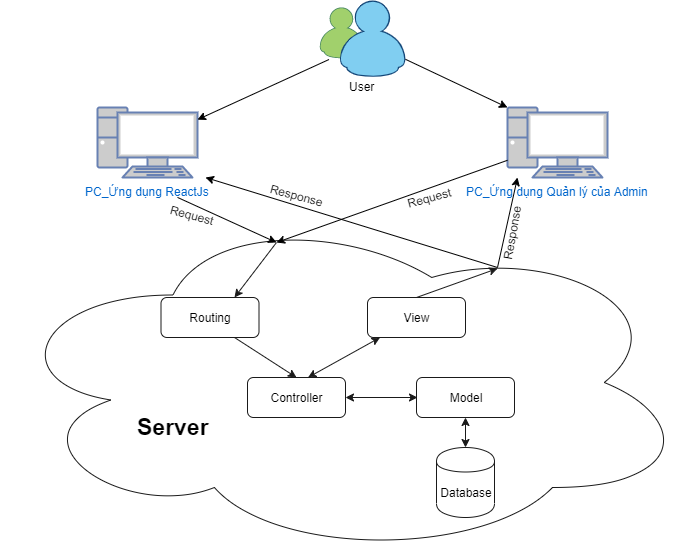
\includegraphics[width=0.75\linewidth,height=9.22cm]{Hinhve/server.png}
    \caption{Mô hình hệ thống dựa theo kiến trúc MVC}
    \label{fig:Fig42}
\end{figure}
Hệ thống được mô tả dựa trên kiến trúc MVC có thêm thành phần Routing có vai trò ánh xạ các request từ phía client đến controller.
\newpage
\subsection{Thiết kế tổng quan}
Mô tả chi tiết các gói trong biểu đồ trên:

Tầng giao diện cho ứng dụng web (FontEndLayer)
\begin{figure}[H]
    \centering
    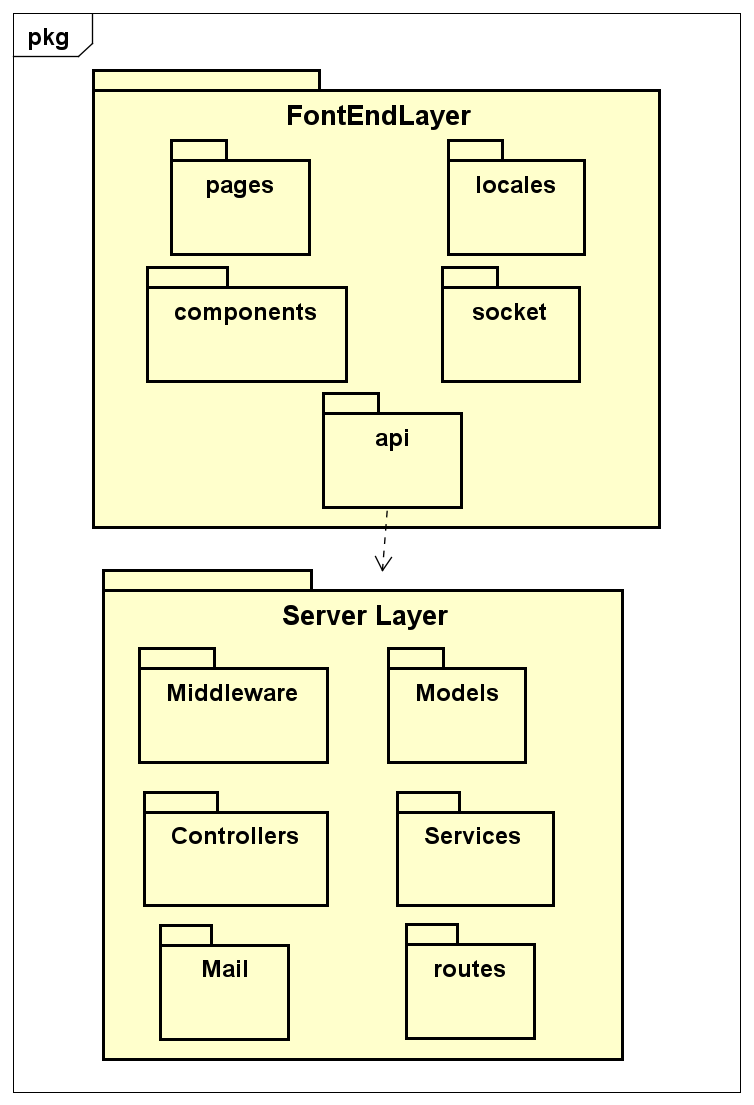
\includegraphics[width=11.4cm,height=16.7cm]{Hinhve/thiet_ke_tong_quan.png}
    \caption{Biểu đồ gói tổng quan}
    \label{fig:Fig43}
\end{figure}
\begin{itemize}
    \item pages: chứa các trang chính của website đấu giá trực tuyến
    \item components: chứa các component có thể tái sử dụng trên toàn website.
    \item locales: chứa các file phục vụ cho việc chuyển đổi ngôn ngữ giữa tiếng Nhật và tiếng Việt
    \item api: chứa các lời gọi RESTful API ở phía Server
    \item socket: có nhiệm vụ trong việc xây dựng tính realtime khi nhắn tin trực tuyến
\end{itemize}
Tầng ứng dụng server (Server Layer)
\begin{itemize}
    \item Middleware: Thành phần có nhiệm vụ đảm bảo người dùng hiện tại có đủ quyền để thực hiện tác vụ nào đó trước khi đưa đến Controllers xử lý.
    \item Controllers: Nhận các request từ phía người dùng. Controller có nhiệm vụ xử lý logic, giao tiếp với Model, nhận dữ liệu từ Model để trả response cho ứng dụng hiển thị lên màn hình.
    \item Models: Có nhiệm vụ định nghĩa cơ sở dữ liệu cho hệ thống, giao tiếp với cơ sở dữ liệu.
    \item Services: Có nhiệm vụ giao tiếp với cơ sở dữ liệu, nhằm giảm tải công việc cho Models.
    \item Mail: Có nhiệm vụ trong việc gửi Mail, khi mà người dùng muốn liên lạc với Admin thông qua Mail.
    \item routers: Có nhiệm vụ phân luồng cho các request gửi đến hệ thống.
    \item view: hiển thị dữ liệu ra màn hình bên hệ thống quản lý của Admin.
\end{itemize}
\subsection{Thiết kế chi tiết gói}
\subsubsection{Thiết kế chi tiết gói cho ứng dụng web ( FontEndLayer)
} \mbox{}
\begin{figure}[H]
    \centering
    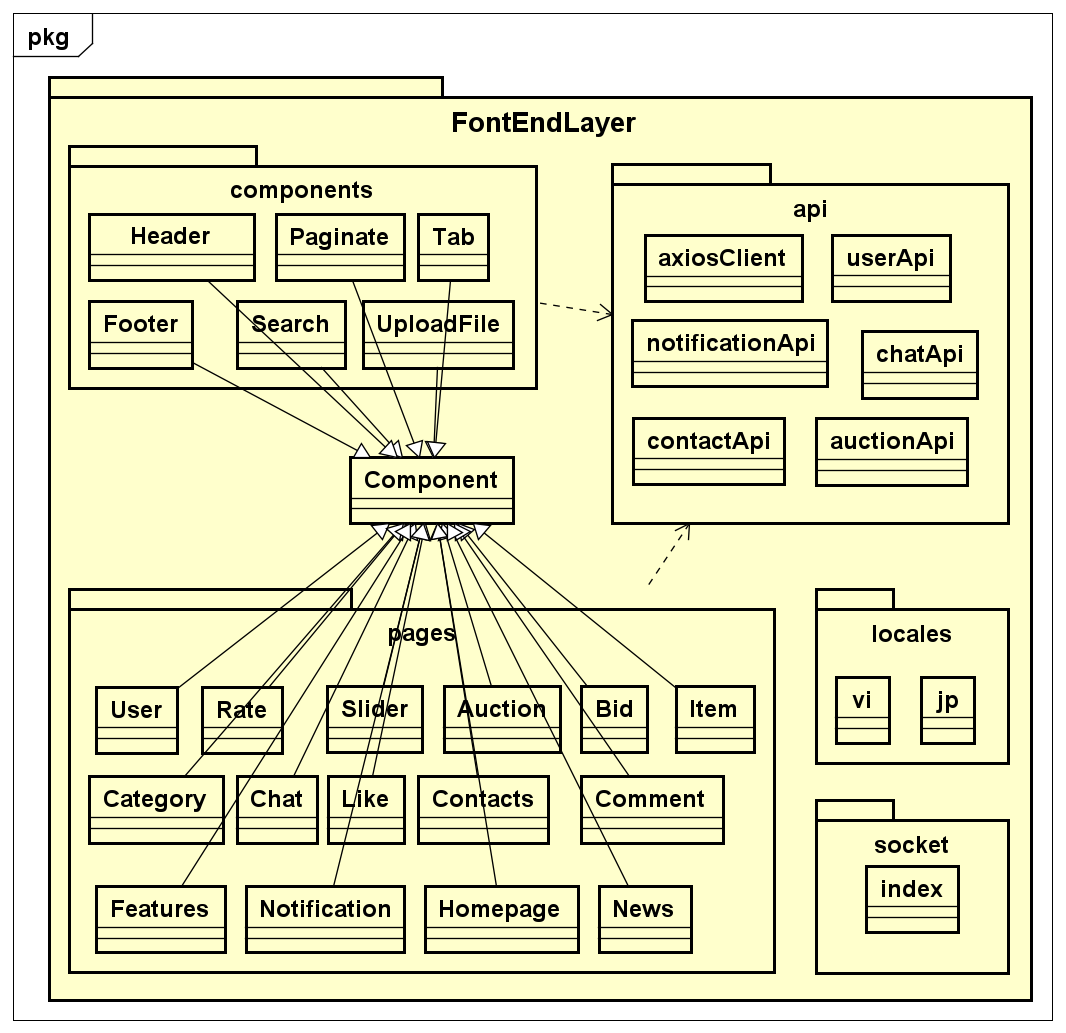
\includegraphics[width=0.75\linewidth,height=10.87cm]{Hinhve/FontEndLayer752.png}
    \caption{Thiết kế chi tiết gói ứng dụng web}
    \label{fig:Fig44}
\end{figure}
Trên ứng dụng web, tất cả các class sẽ được kết thừa từ Component của ReactJs.\\
Mỗi gói sẽ có một nhiệm vụ khác nhau: \\
Gói components sẽ chứa các thành phần có khả năng tái sử dụng trên toàn bộ website.
\begin{itemize}
    \item Footer: giao diện chân trang của tất cả các màn hình.
    \item Header: giao diện thanh header hiển thị bên trên tất cả các màn hình.
    \item Paginate: giao diện thanh phân trang ở tất cả các màn liệt kê danh sách.
    \item Search: giao diện thanh tìm kiếm.
    \item Tab: Giao diện thanh chia danh sách phiên đấu giá theo trạng thái.
\end{itemize}
Gói pages chứa thành phần hiển thị trên màn hình client của website đấu giá trực tuyến.
\begin{itemize}
    \item HomePage: giao diện trang chủ.
    \item Features: danh sách phiên đấu giá tại trang chủ.
    \item Slider: slide hiển thị tại trang chủ.
    \item Category: danh sách loại sản phẩm tại trang chủ.
    \item News: giao diện liên quan đến bản tin (danh sách, chi tiết bản tin).
    \item Contacts: giao diện khi liên lạc với Admin qua email.
    \item Notifications: giao diện thông báo (danh sách, chi tiết thông báo).
    \item User: giao diện liên quan đến Người dùng (đăng nhập, đăng ký, thay đổi mật khẩu, chỉnh sửa tài khoản).
    \item Auction: giao diện liên quan đến phiên đấu giá (thêm, sửa, danh sách, chi tiết phiên đấu giá).
    \item Item: giao diện liên quan đến sản phẩm của phiên đấu giá (thêm, sửa, chi tiết sản phẩm của phiên đấu giá).
    \item Bid: giao diện liên quan đến trả giá (thêm, danh sách trả giá).
    \item Comment: giao diện liên quan đến bình luận (thêm, xóa, danh sách bình luận).
    \item Rate: giao diện đánh giá sản phẩm khi nhận được hàng.
    \item Chat: giao diện màn hình nhắn tin.
    \item Like: giao diện thích một phiên đấu giá (yêu thích, danh sách yêu thích).
\end{itemize}
Gói api chứa các lời gọi RESTful API từ server.
\begin{itemize}
    \item axiosClient: định dạng chung lời gọi RESTful API.
    \item userApi: lời gọi RESTful API liên quan đến người dùng.
    \item auctionApi: lời gọi RESTful API liên quan đến phiên đấu giá.
    \item notificationApi: lời gọi RESTful API liên quan đến thông báo.
    \item chatApi: lời gọi RESTful API liên quan đến nhắn tin.
    \item contactApi: lời gọi RESTful API liên quan đến liên lạc với Admin bằng email.
\end{itemize}
Gói locales chứa các file phục vụ cho việc chuyển đổi giữa tiếng Nhật và tiếng Việt.
\begin{itemize}
    \item jp: lưu trữ các key và text bằng tiếng Nhật tương ứng.
    \item vi: lưu trữ các key và text bằng tiếng Việt tương ứng.
\end{itemize}
Gói socket được gọi khi người dùng truy cập vào ứng dụng chat. Gói socket đảm bảo ứng dụng chat hoạt động realtime.
\subsubsection{Thiết kế chi tiết gói cho server (ServerLayer)}
\begin{figure}[H]
    \centering
    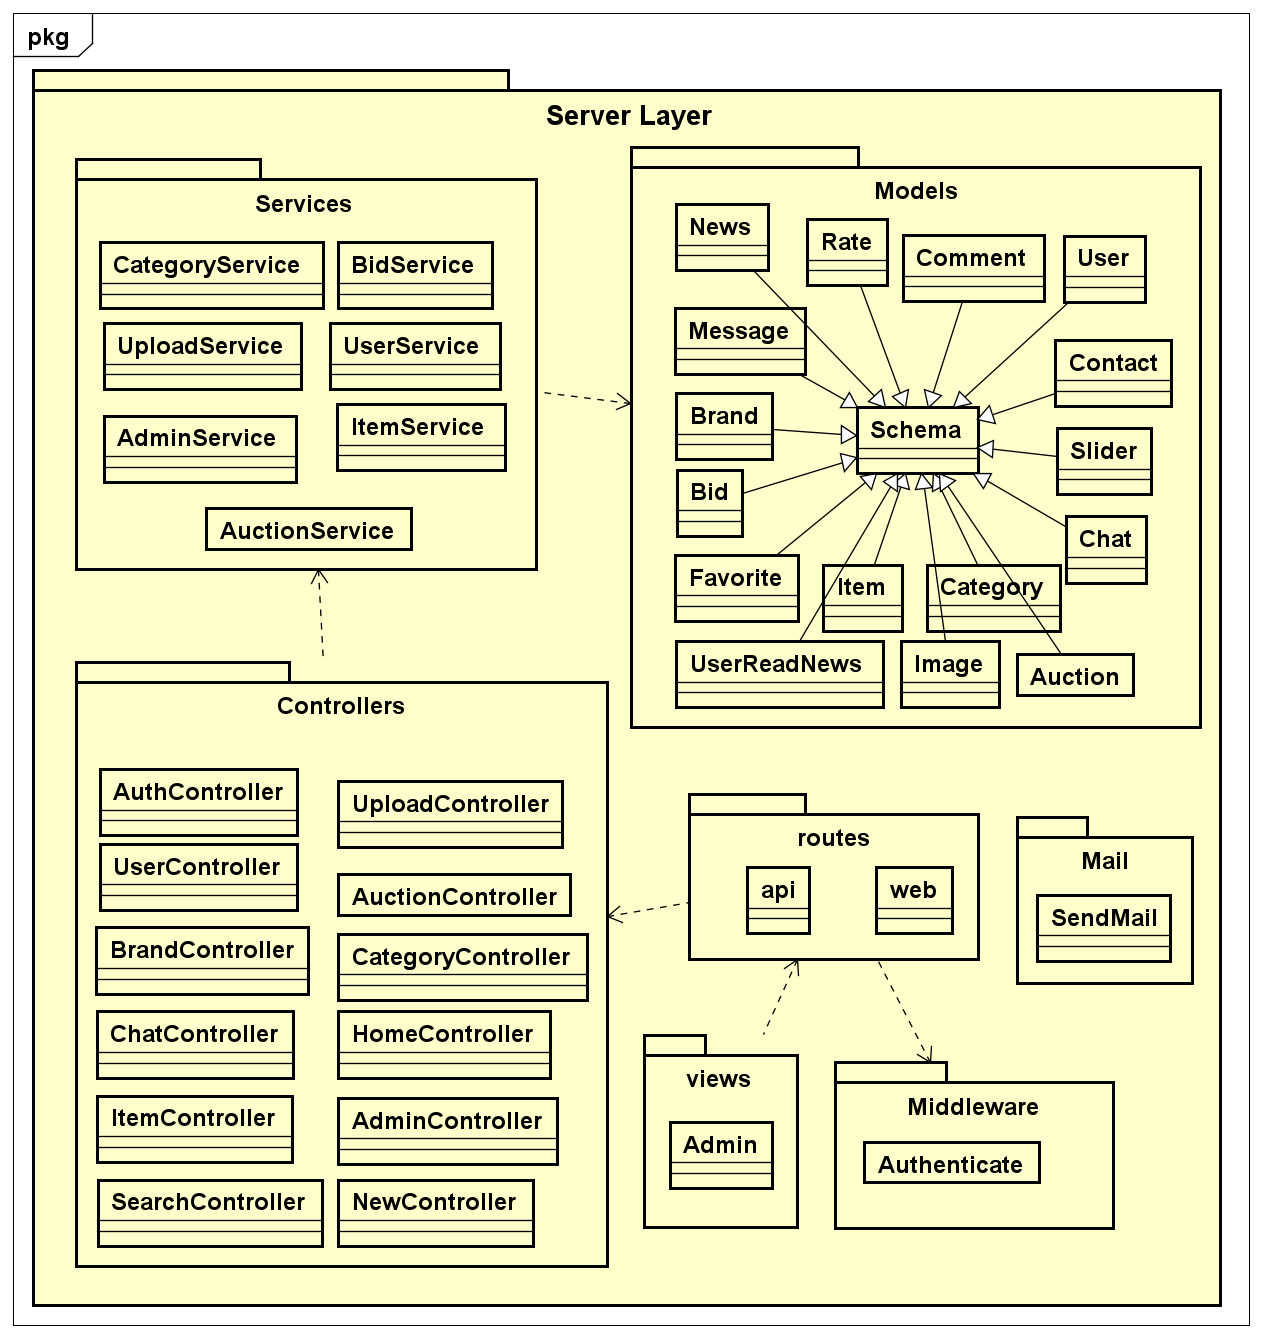
\includegraphics[width=0.75\linewidth,height=11.9cm]{Hinhve/ServerLayer75.png}
    \caption{Thiết kế chi tiết gói serverlayer}
    \label{fig:Fig45}
\end{figure}
Sau khi phía client gọi các RESTful API, hệ thống sẽ gửi request về cho controller phía trong gói Server Layer. Sau khi nhận được lời gọi thì phía controller sẽ gọi đến middleware để kiểm tra người dùng truy cập có đáp ứng điều kiện để thông qua không. Nếu thông qua middleware, thì dựa vào request được gửi tới, controller sẽ vào các model, service để lấy dữ liệu tương ứng rồi trả về cho client.\\ 
Sau đây là mô tả chi tiết các class có trong ServerLayer:\\
Gói routes có nhiệm vụ xử lý phân luồng cho các request gửi đến hệ thống:
\begin{itemize}
    \item api: chứa các đường dẫn api xử lý phía client.
    \item web: chứa các đường dẫn xử lý phía admin.
\end{itemize}
Gói controllers:
\begin{itemize}
    \item AuthController: Xử lý các API liên quan đến việc xác minh tài khoản người dùng.
    \item UserController: Xử lý các API liên quan đến tài khoản người dùng.
    \item AuctionController: Xử lý các API liên quan đến phiên đấu giá.
    \item ItemController: Xử lý các API liên quan đến sản phẩm.
    \item BrandController: Xử lý các API liên quan đến thương hiệu.
    \item CategoryController: Xử lý các API liên quan đến loại sản phẩm.
    \item ChatController: Xử lý các API liên quan đến nhắn tin.
    \item NewController: Xử lý các API liên quan đến tin tức.
    \item UploadController: Xử lý các API liên quan đến upload hình ảnh.
    \item SearchController: Xử lý các API liên quan đến tìm kiếm.
    \item HomeController: Xử lý các API liên quan đến trang chủ (slide).
    \item AdminController: Xử lý các sự kiện phía quản trị viên.
\end{itemize}
Gói models:
\begin{itemize}
    \item User: định nghĩa dữ liệu cho bảng users và quan hệ với các bảng khác trong cơ sở dữ liệu.
    \item Auction: định nghĩa dữ liệu cho bảng auctions và quan hệ với các bảng khác trong cơ sở dữ liệu.
    \item Item: định nghĩa dữ liệu cho bảng items và quan hệ với các bảng khác trong cơ sở dữ liệu.
    \item Image: định nghĩa dữ liệu cho bảng images và quan hệ với các bảng khác trong cơ sở dữ liệu.
    \item Category: định nghĩa dữ liệu cho bảng categories và quan hệ với các bảng khác trong cơ sở dữ liệu.
    \item Brand: định nghĩa dữ liệu cho bảng brands và quan hệ với các bảng khác trong cơ sở dữ liệu.
    \item Bid: định nghĩa dữ liệu cho bảng bids và quan hệ với các bảng khác trong cơ sở dữ liệu.
    \item Comment: định nghĩa dữ liệu cho bảng comments và quan hệ với các bảng khác trong cơ sở dữ liệu.
    \item News: định nghĩa dữ liệu cho bảng news và quan hệ với các bảng khác trong cơ sở dữ liệu.
    \item UserReadNews: định nghĩa dữ liệu cho bảng user\_read\_news và quan hệ với các bảng khác trong cơ sở dữ liệu.
    \item Contact: định nghĩa dữ liệu cho bảng contacts và quan hệ với các bảng khác trong cơ sở dữ liệu.
    \item Slider: định nghĩa dữ liệu cho bảng sliders và quan hệ với các bảng khác trong cơ sở dữ liệu.
    \item Favorites: định nghĩa dữ liệu cho bảng favorites và quan hệ với các bảng khác trong cơ sở dữ liệu.
    \item Chat: định nghĩa dữ liệu cho bảng chat và quan hệ với các bảng khác trong cơ sở dữ liệu.
    \item Message: định nghĩa dữ liệu cho bảng messages và quan hệ với các bảng khác trong cơ sở dữ liệu.
    \item Rate: định nghĩa dữ liệu cho bảng rate và quan hệ với các bảng khác trong cơ sở dữ liệu.
\end{itemize}
Gói services có nhiệm vụ giao tiếp với cơ sở dữ liệu (nhằm giảm tải công việc của Models):
\begin{itemize}
    \item UserService: xử lý các function thao tác với cơ sở dữ liệu liên quan đến người dùng.
    \item AuctionService: xử lý các function thao tác với cơ sở dữ liệu liên quan đến phiên đấu giá.
    \item ItemService: xử lý các function thao tác với cơ sở dữ liệu liên quan đến sản phẩm.
    \item CategoryService: xử lý các function thao tác với cơ sở dữ liệu liên quan đến loại sản phẩm.
    \item BidService: xử lý các function thao tác với cơ sở dữ liệu liên quan đến trả giá.
    \item UploadService: xử lý các function thao tác với cơ sở dữ liệu liên quan đến upload hình ảnh.
    \item AdminService: xử lý các function thao tác với cơ sở dữ liệu liên quan đến hệ thống quản trị viên.
\end{itemize}
Gói views: 
\begin{itemize}
    \item Admin: gồm các trang quản lý dành cho quản trị viên.
\end{itemize}
\section{Thiết kế chi tiết}
\subsection{Thiết kế giao diện}
Trong phần này đồ án sẽ trình bày về các nguyên tắc chung khi thiết kế giao diện  và phác thảo một số màn hình chính, các thông số quan trọng của màn hình trong website đấu giá trực tuyến.
\subsubsection{Thông số màn hình}
%\begin{table}[]
    %\centering
    \tablehead{%
    \hline
    \bfseries STT & \bfseries Thông tin & \bfseries Các thông số màn hình  \\\hline}
    \tabletail{\hline}
    \topcaption{Thông số màn hình trong thiết kế giao diện ứng dụng web của client}
    \label{bang41}
    \begin{supertabular}{| p{.05\textwidth} | p{.30\textwidth} | p{.55\textwidth} |} 
        1 & Kích thước màn hình &
            \begin{tabular}{p{.45\textwidth}}
                Máy tính bàn : \\
                (Desktops - Medium devices): >= 992px\\
                Máy tính lớn : \\
                (Large Desktops - Large devices) >= 1200px
            \end{tabular}\\\hline
        2 & Màu sắc &
            \begin{tabular}{p{.45\textwidth}}
                Màu nền: \#F8F9FA\\
                Màu tiêu đề: màu xanh \#7FAD39 hoặc màu đen \#000000\\
                Màu chữ thường: màu đen \#000000\\
                Màu liên kết: màu xanh nhạt \#E6EFE6, khi di chuyển chuột vào thì thành màu xanh đậm hơn một chút \#F8F9FA
            \end{tabular}\\\hline
        3 & Kiểu chữ &
        Segoe UI
        \\\hline
        4 & Ngôn ngữ &
        Tiếng Việt, Tiếng Nhật
        \\\hline
    \end{supertabular}\\
% \end{table}
\\
%\begin{table}[H]
    %\centering
     \tablehead{%
    \hline
    \bfseries STT & \bfseries Thông tin & \bfseries Các thông số màn hình  \\\hline}
    \tabletail{\hline}
    \topcaption{Thông số màn hình trong thiết kế giao diện ứng dụng web của hệ thống admin}
    \label{bang42}
    \begin{supertabular}{| p{.05\textwidth} | p{.30\textwidth} | p{.55\textwidth} |} 
    \hline
        1 & Kích thước màn hình &
            \begin{tabular}{p{.45\textwidth}}
                Máy tính bàn\\
                (Desktops - Medium devices): >= 992px\\
                Máy tính lớn\\
                (Large Desktops - Large devices) 
                >= 1200px\\
                Di động: (Phones) <=768px\\
            \end{tabular}
        \\\hline
        2 & Màu sắc &
            \begin{tabular}{p{.45\textwidth}}
                Màu nền: xám trắng \#F8F9FA\\
                Màu tiêu đề: màu đen \#000000\\
                Màu chữ thường: màu đen \#000000 hoặc màu trắng \#fff\\
                Màu liên kết:  màu xanh nước biển \#007bff\\
            \end{tabular}
        \\\hline
        3 & Theme &
        AdminLTE
        \\\hline
        4 & Kiểu chữ &
        Segoe UI
        \\\hline
        5 & Ngôn ngữ &
        Tiếng Việt, Tiếng Nhật
        \\\hline
    \end{supertabular}
%\end{table}
\subsubsection{Nguyên tắc thiết kế chung}
Mục tiêu của website là đáp ứng được yêu cầu dễ sử dụng, thân thiện với người dùng. Vì vậy đồ án phải đảm bảo khi người dùng nhìn vào sẽ biết chức năng của từng nút, nắm cơ bản luồng hoạt động của ứng dụng. Người dùng có thể dự đoán được nếu nhấn nút này hay bỏ qua trường này thì sẽ có điều gì xảy ra tiếp theo. Ví dụ ở các form đăng ký thì những trường bắt buộc sẽ được đánh dấu sao màu đỏ, thông báo đầy đủ lỗi khi người dùng nhập thông tin không phù hợp, các trường cần bảo mật thì ẩn thông tin khi nhập xong. Đặc biệt khi người dùng muốn xóa gì đó thì cần phải xác nhận lại thông tin, đảm bảo hành vi không phải là vô tình. Sau khi người dùng thực hiện xong các thao tác thì thông báo bằng các toast màu sắc phù hợp để dễ dàng nhận biết là tác vụ đã thành công hay chưa. 

Ngoài ra để đảm bảo người dùng không cảm thấy khó chịu khi sử dụng website thì màu sắc của giao diện cũng cần được thống nhất, chọn tông màu sáng, nhẹ nhàng, không cho quá nhiều màu sắc sặc sỡ. Với các thông báo thì cần dùng màu sắc đặc trưng hay được dùng nhiều như tác vụ thành công màu \#28A475 (\textbf{success}), lỗi màu \#DC3545 (\textbf{error}), cảnh báo màu \#FFC107 (\textbf{warning}). Đối với các tác vụ mà có thể click chuột được thì khi di chuyển chuột vào sẽ phải thay đổi màu sắc để người dùng dễ nhận biết. Với các hộp thông báo thì hiển thị giữa màn hình, các thông tin bên dưới làm mờ để nổi bật hộp thông báo.
\subsubsection{Thiết kế sơ đồ hệ thống}
Sau đây đồ án sẽ trình bày sơ đồ màn hình của hệ thống phía Người dùng và hệ thống quản trị phía Quản trị viên.
\begin{figure}[H]
    \centering
    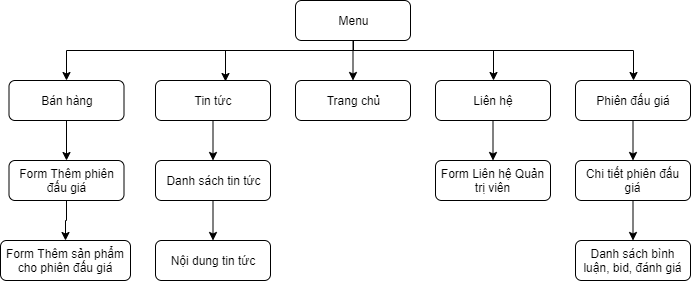
\includegraphics[width=0.75\linewidth,height=4.65cm]{Hinhve/clientpage.png}
    \caption{Sơ đồ hệ thống phía Người dùng}
    \label{fig:Fig46}
\end{figure}
Sơ đồ trên thể hiện phía giao diện Người dùng có 5 giao diện chính, (i) Bán hàng: khi người dùng muốn tạo một phiên đấu giá thì sẽ thực hiện ở màn hình này, (ii) Bài viết : Hiển thị những bài viết, tin tức mà phía Quản trị viên thêm vào, (iii) Trang chủ:  Hiển thị danh sách các phiên đấu giá của toàn hệ thống, (iv) Liên hệ: khi người dùng muốn liên hệ với Quản trị viên qua email. Cuối cùng là Phiên đấu giá bao gồm chi tiết phiên đấu giá và danh sách các bình luận, trả giá (bid), đánh giá của người dùng.
\begin{figure}[H]
    \centering
    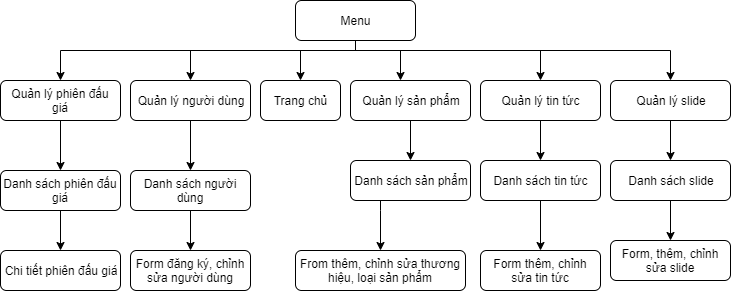
\includegraphics[width=0.75\linewidth,height=4.54cm]{Hinhve/adminpage.png}
    \caption{Sơ đồ hệ thống phía Quản trị viên}
    \label{fig:Fig47}
\end{figure}
Phía Quản trị viên có 6 giao diện chính trang chủ, quản lý phiên đấu giá, người dùng, sản phẩm, tin tức và slide.
\newpage
\subsubsection{Thiết kế phác thảo màn hình chính}
Sau đây là mockup một số màn hình chính (i) giao diện trang chủ, (ii) giao diện tạo phiên đấu giá, (iii) giao diện thêm sản phẩm cho phiên đấu giá, (iv) giao diện chi tiết phiên đấu giá
\begin{figure}[H]
    \centering
    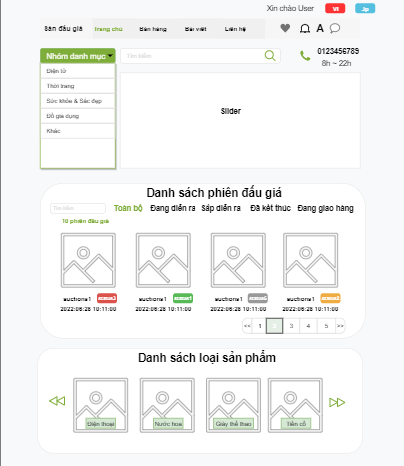
\includegraphics[width=0.75\linewidth,height=14.5cm]{Hinhve/homepage.png}
    \caption{Mockup màn hình trang chủ}
    \label{fig:Fig48}
\end{figure}
Hình \ref{fig:Fig48} mô tả mockup giao diện màn hình trang chủ phía Người dùng. Phần header bao gồm tên tài khoản đang đăng nhập, icon chuyển đổi giữa tiếng Việt và Tiếng Nhật; tiếp theo là thanh navbar chứa tiêu đề của các page chính và icon liên quan (icon tim liên kết đến danh sách phiên đấu giá yêu thích, icon chuông liên kết đến danh sách thông báo, icon A liên kết đến trang cá nhân của người dùng, icon tin nhắn liên kết đến ứng dụng chat realtime). Tiếp đến website hiển thị nhóm danh mục loại sản phẩm, thanh tìm kiếm, slide hiển thị trên trang chủ, số điện thoại và thời gian mà admin có thể hỗ trợ. Trang chủ cũng hiển thị danh sách toàn bộ phiên đấu giá, loại sản phẩm hiện có trên toàn hệ thống. Phần footer chứa thông tin, địa chỉ, các tài khoản xã hội của website.
\begin{figure}[H]
    \centering
    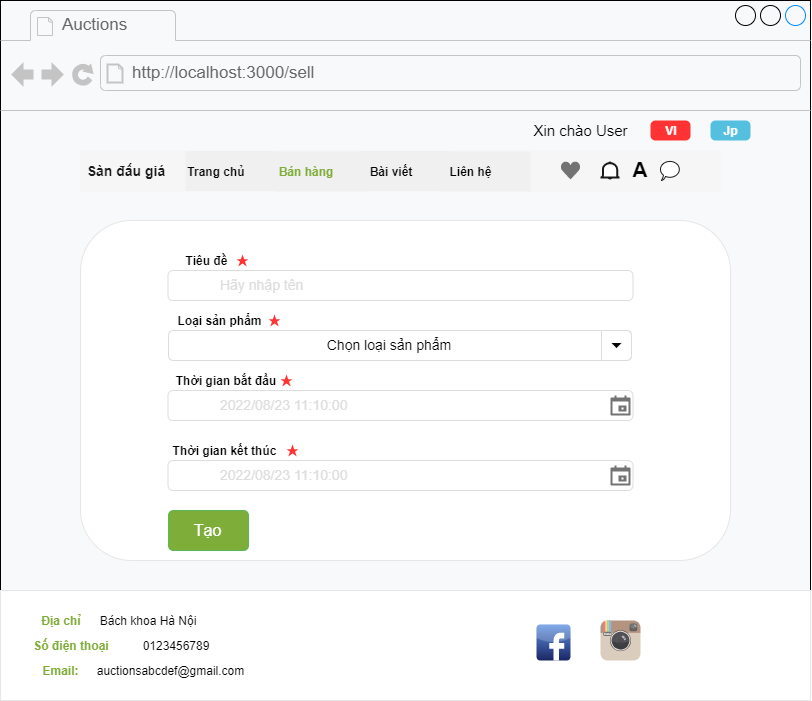
\includegraphics[width=0.75\linewidth,height=9.7cm]{Hinhve/createauction.png}
    \caption{Mockup màn hình tạo phiên đấu giá}
    \label{fig:Fig49}
\end{figure}
Hình \ref{fig:Fig49} mô tả mockup giao diện tạo một phiên đấu giá. Những trường nào yêu cầu phải nhập sẽ có hình ngôi sao màu đỏ để người dùng dễ nhận biết.
\newpage
\begin{figure}[H]
    \centering
    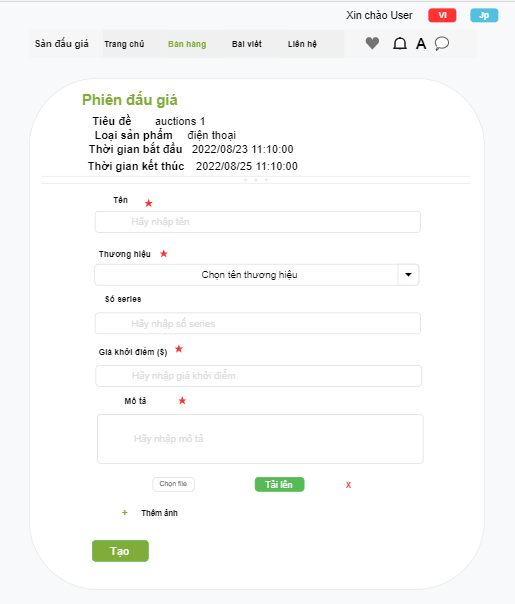
\includegraphics[width=0.75\linewidth,height=13.08cm]{Hinhve/itemcreate.png}
    \caption{Mockup màn hình Tạo sản phẩm cho phiên đấu giá}
    \label{fig:Fig410}
\end{figure}
Hình \ref{fig:Fig410} mô tả mockup giao diện màn hình tạo sản phẩm cho một phiên đấu giá. Phía trên cùng là thông tin phiên đấu giá mà người dùng đang thêm sản phẩm. phía dưới là form để điền các thông tin của sản phẩm cần thêm. Đồng tiền được quy định chung cho website là \$ (đô la).
\newpage
\begin{figure}[H]
    \centering
    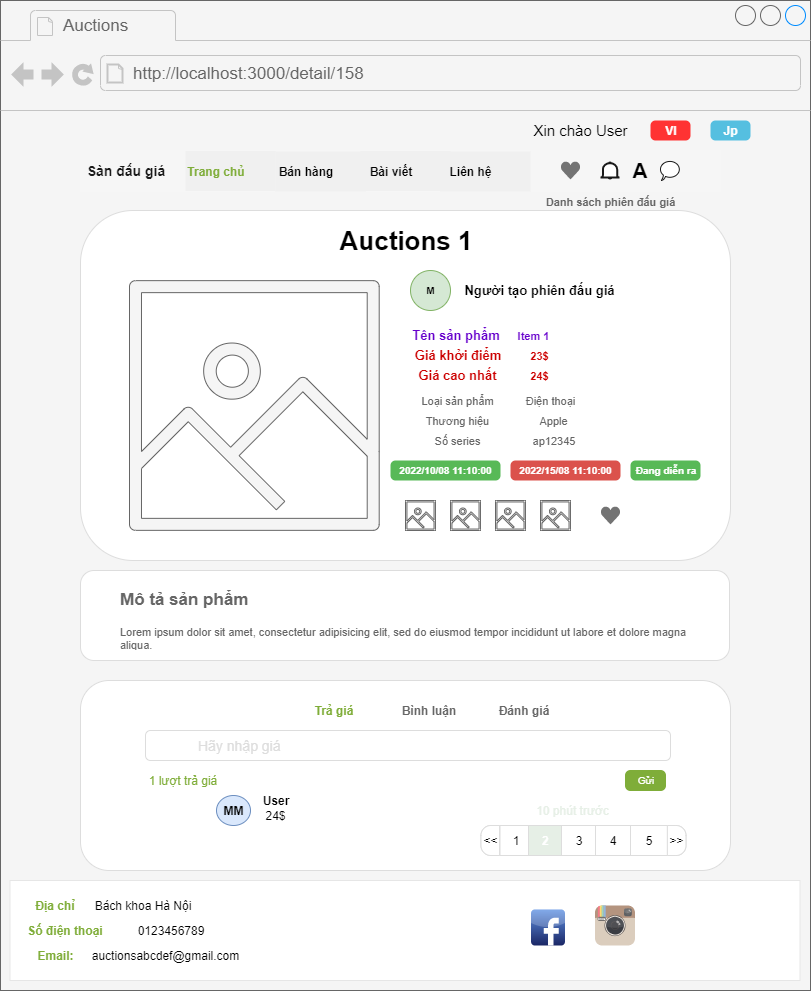
\includegraphics[width=0.75\linewidth,height=13.1cm]{Hinhve/detailitem.png}
    \caption{Mockup màn hình Chi tiết phiên đấu giá}
    \label{fig:Fig411}
\end{figure}
Hình \ref{fig:Fig411} mô tả giao diện của màn hình chi tiết phiên đấu giá, bao gồm các hình ảnh, trạng thái phiên đấu giá, thông tin của sản phẩm, avatar, tên của người tạo phiên đấu giá. Phía dưới là các tab để trả giá, bình luận, đánh giá sản phẩm. 
\newpage
\subsection{Thiết kế lớp}
\begin{figure}[H]
    \centering
    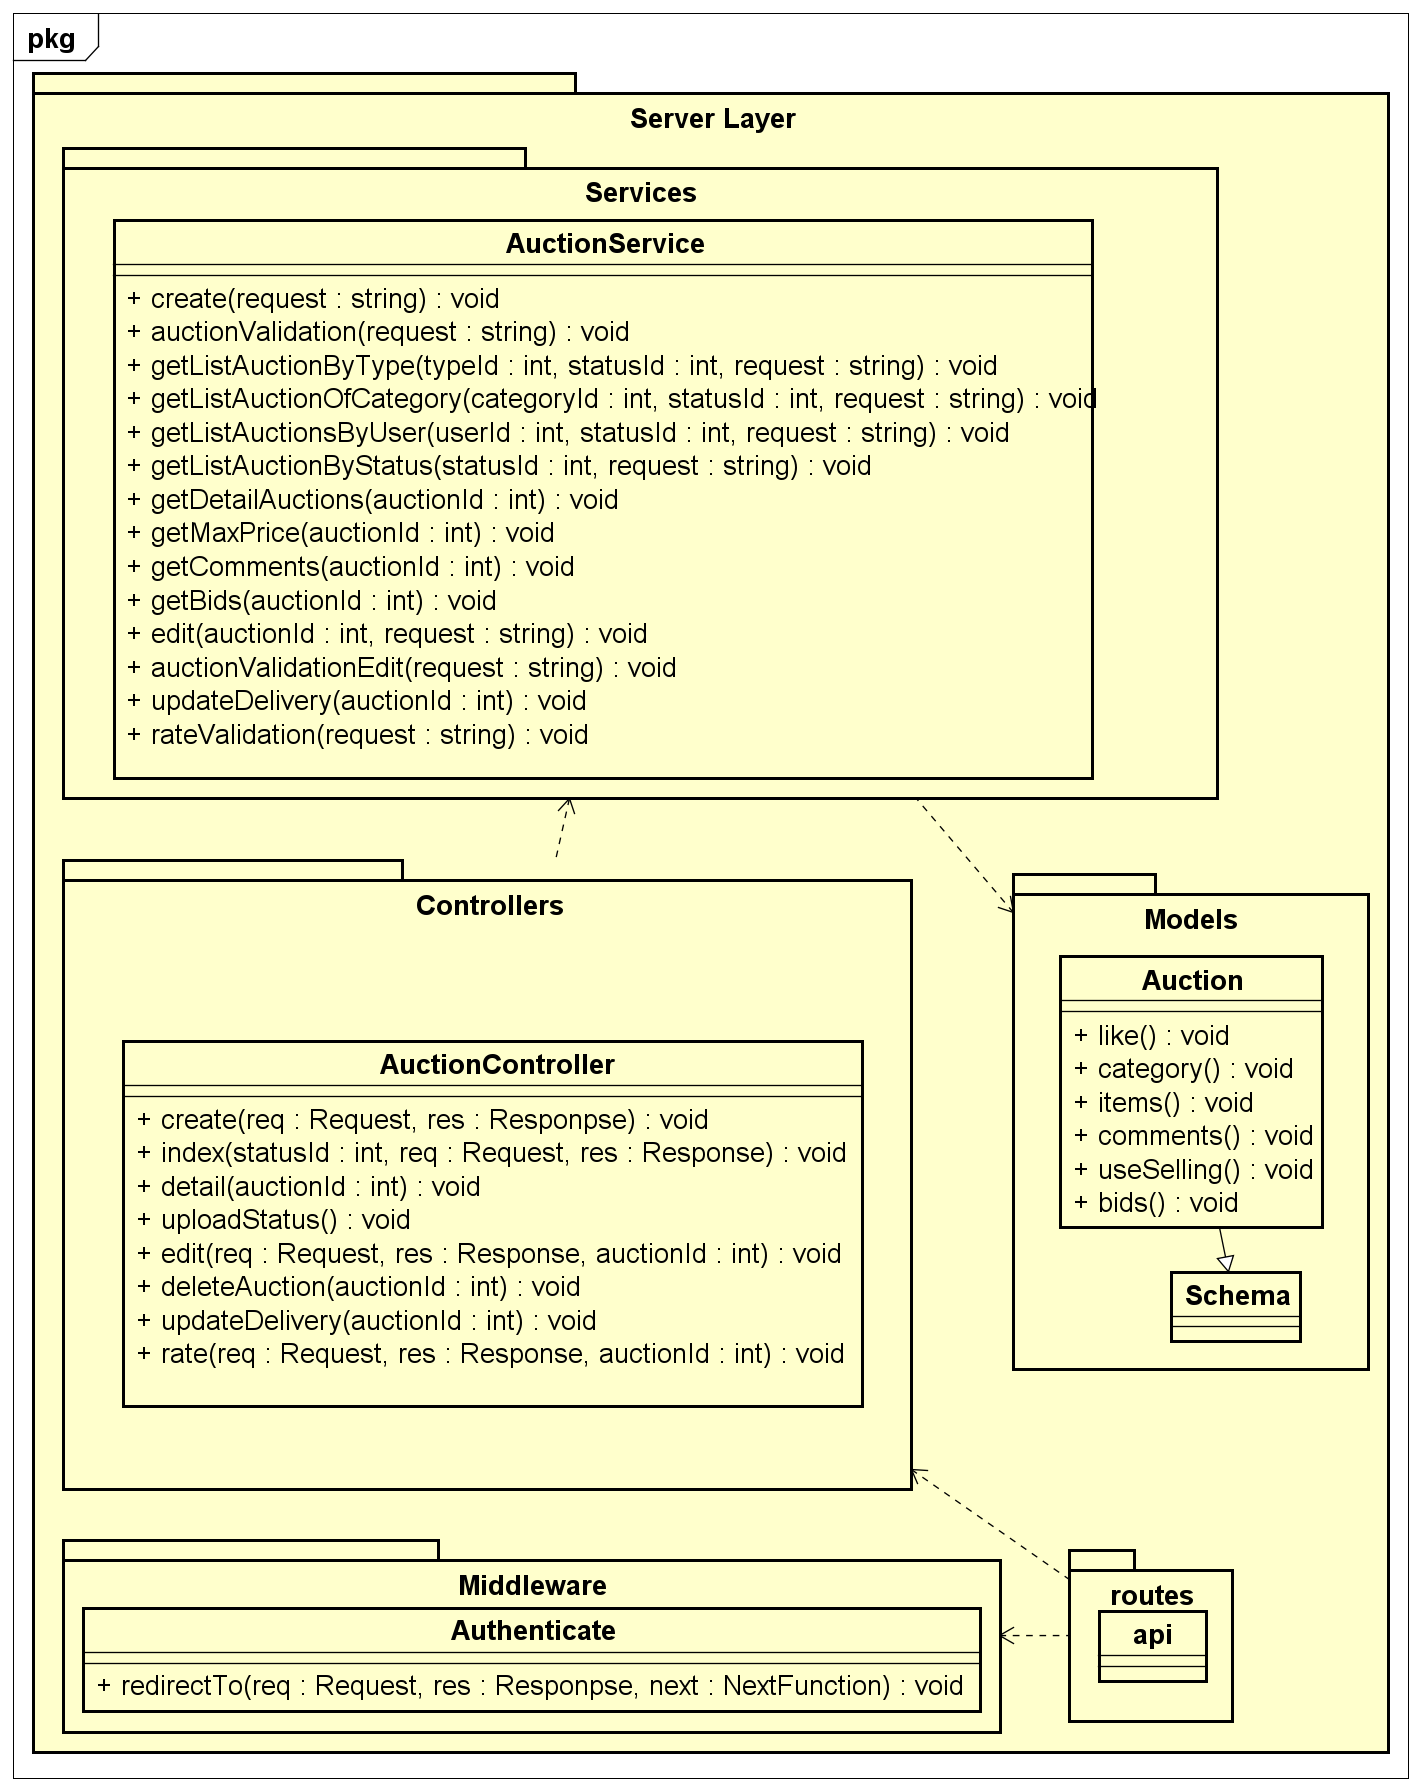
\includegraphics[width=0.75\linewidth,height=13.74cm]{Hinhve/Thiết kế chi tiết75.png}
    \caption{Thiết kế lớp quản lý phiên đấu giá}%( tạo, chỉnh sửa, xóa, cập nhật trạng thái, giao hàng, đánh giá)
    \label{fig:Fig412}
\end{figure}

%\begin{table}[]
    %\centering
    \begin{longtable}{| p{.20\textwidth} | p{.20\textwidth} | p{.10\textwidth} | p{.40\textwidth} |}
    \caption{Bảng đặc tả lớp Authenticate}
    \label{bang43}
    \endfirsthead
    \endhead
    \hline
        \bfseries Tên phương thức & \bfseries Đầu vào & \bfseries Đầu ra & \bfseries Ý nghĩa\\\hline
        \multicolumn{4}{|c|}{Lớp Authenticate}\\\hline
        redirectTo & {%
            \begin{tabular}{l}
                 Request\\
                 Response\\
                 NextFunction
            \end{tabular}
        } & void &  Hàm xử lý request khi tài khoản người dùng cần phải đăng nhập thì mới được sử dụng các tác vụ sau. Nếu chưa đăng nhập thì trả message “Chưa đăng nhập”\\\hline
    \end{longtable}\\
% \end{table}

%\begin{table}[H]
    %\centering
    \tablehead{%
    \hline
    \bfseries Tên phương thức & \bfseries Đầu vào & \bfseries Đầu ra & \bfseries Ý nghĩa  \\\hline}
    \tabletail{\hline}
    \topcaption{Bảng đặc tả lớp AuctionController}
    \label{bang44}
    \begin{supertabular}{| p{.20\textwidth} | p{.15\textwidth} | p{.15\textwidth} | p{.40\textwidth} |}
    \hline
        \multicolumn{4}{|c|}{Lớp AuctionController}\\\hline
        create & Request, Response & void & Hàm tạo phiên đấu giá\\\hline
        index & statusId, Request, Response & void & Hàm lấy ra danh sách phiên đấu giá theo trạng thái (statusId)\\\hline
        detail & auctionId & void & Hàm lấy ra chi tiết phiên đấu giá\\\hline
        uploadStatus & & void & Hàm cập nhật trạng thái phiên đấu giá\\\hline
        edit & auctionId, Request, Response & void & Hàm chỉnh sửa phiên đấu giá chưa được duyệt\\\hline
        deleteAuction & auctionId & void & Hàm xóa phiên đấu giá chưa được duyệt\\\hline
        updateDelivery & auctionId & void & Hàm update tình trạng giao hàng\\\hline
        rate & auctionId, Request, Response & void & Hàm đánh giá sản phẩm của phiên đấu giá\\\hline
    \end{supertabular}
%\end{table}
%\begin{table}[H]
    %\centering
    \tablehead{%
    \hline
    \bfseries Tên phương thức & \bfseries Đầu vào & \bfseries Đầu ra & \bfseries Ý nghĩa  \\\hline}
    \tabletail{\hline}
    \topcaption{Bảng đặc tả lớp AuctionService}
    \label{bang45}
    \begin{supertabular}{| p{.32\textwidth} | p{.14\textwidth} | p{.14\textwidth} | p{.30\textwidth} |} 
    \hline
        \multicolumn{4}{|c|}{Lớp AuctionService}\\\hline
        create & request & void & Hàm tạo phiên đấu giá\\\hline
        auctionValidation & request & void & Hàm để bắt các lỗi khi tạo phiên đấu giá\\\hline
        getListAuctionByType & typeId, satusId, request & void & Hàm lấy ra chi tiết phiên đấu giá theo trạng thái (statusId) và nhóm loại sản phẩm (typeId)\\\hline
        getListAuctionOfCategory & & categoryId, statusId, request & Hàm lấy ra chi tiết phiên đấu giá theo trạng thái (statusId) và loại sản phẩm (categoryId)\\\hline
        getListAuctionByUser & userId, satusId, request& void & Hàm lấy ra chi tiết phiên đấu giá theo trạng thái (statusId) và người dùng (userId)\\\hline
        getListAuctionStatus & statusId, request & void & Hàm lấy ra chi tiết phiên đấu giá theo trạng thái (statusId) trên toàn hệ thống\\\hline
        getDetailAuctions & auctionId & void & Chi tiết phiên đấu giá\\\hline
        getMaxPrice & auctionId & void & Hàm trả về lượt trả giá cao nhất của phiên đấu giá\\\hline
        getComments & auctionId & void & Hàm trả về danh sách bình luận của phiên đấu giá\\\hline
        getBids & auctionId & void & Hàm trả về danh sách trả giá của phiên đấu giá\\\hline
        getMaxPrice & auctionId, Request, Response & void & Hàm đánh giá sản phẩm phiên đấu giá\\\hline
        edit & auctionId, request & void & Hàm chỉnh sửa phiên đấu giá chưa được duyệt\\\hline
        auctionValidationEdit & request & void & Hàm bắt lỗi khi chỉnh sửa phiên đấu giá chưa được duyệt\\\hline
        updateDelivery & request & void & Cập nhật trạng thái giao hàng\\\hline
        rateValidation & auctionId & void & Bắt lỗi khi đánh giá sản phẩm của phiên đấu giá sau khi nhận được hàng.\\\hline
    \end{supertabular}
%\end{table}
%\begin{table}[H]
    %\centering
    \tablehead{%
    \hline
    \bfseries Tên phương thức & \bfseries Đầu vào & \bfseries Đầu ra & \bfseries Ý nghĩa  \\\hline}
    \tabletail{\hline}
    \topcaption{Bảng đặc tả lớp Auction}
    \label{bang46}
    \begin{supertabular}{| p{.20\textwidth} | p{.15\textwidth} | p{.15\textwidth} | p{.40\textwidth} |} 
    \hline
        \multicolumn{4}{|c|}{Lớp Auction}\\\hline
        like & & void & Hàm định nghĩa quan hệ giữa bảng auctions và favorites\\\hline
        category & & void & Hàm định nghĩa quan hệ giữa bảng auctions và categories\\\hline
        items & & void & Hàm định nghĩa quan hệ giữa bảng auctions và items\\\hline
        comments & & void & Hàm định nghĩa quan hệ giữa bảng auctions và comments\\\hline
        useSelling & & void & Hàm định nghĩa quan hệ giữa bảng auctions và users\\\hline
        bids & & void & Hàm định nghĩa quan hệ giữa bảng auctions và bids\\\hline
    \end{supertabular}
%\end{table}
\subsection{Thiết kế API}
Phần này sẽ liệt kê danh sách các API sử dụng trong hệ thống.
%\begin{table}[H]
    %\centering
    \tablehead{%
    \hline
    \bfseries STT & \bfseries Mục đích & \bfseries Phương thức & \bfseries Địa chỉ  \\\hline}
    \tabletail{\hline}
    \topcaption{Danh sách API}
    \label{bang47}
    \begin{supertabular}{| p{.05\textwidth} | p{.30\textwidth} | p{.10\textwidth} | p{.45\textwidth} |} 
    \hline
        1 & Đăng nhập & POST & /api/login\\\hline
        2 & Đăng ký & POST & /api/signup\\\hline
        3 & Chỉnh sửa tài khoản & POST & /api/edit\\\hline
        4 & Thay đổi mật khẩu & POST & /api/changepass\\\hline
        5 & Đăng xuất & POST & /api/logout\\\hline
        6 & Thông tin tài khoản & GET & /api/info\\\hline
        7 & Danh sách phiên đấu giá & GET & /api/auctions/{statusId}\\\hline
        8 & Chi tiết phiên đấu giá & GET & /api/auctions/detail/{auctionId}\\\hline
        9 & Tạo phiên đấu giá & POST & /api/auctions/create\\\hline
        10 & Chỉnh sửa phiên đấu giá chưa được duyệt & POST & /api/auctions/edit/{auctionId}\\\hline
        11 & Xóa phiên đấu giá chưa được duyệt & POST & /api/auctions/deleteAuction/{auctionId}\\\hline
        12 & Thêm sản phẩm cho phiên đấu giá & POST & /api/items/create/{auctionId}\\\hline
        13 & Chỉnh sửa sản phẩm của phiên đấu giá chưa được duyệt & POST & /api/items/edit/{auctionId}\\\hline
        14 & Danh sách bình luận của phiên đấu giá & GET & /api/comments/{auctionId}\\\hline
        15 & Bình luận & POST & /api/comments/create/{auctionId}\\\hline
        16 & Xóa bình luận & POST & /api/comments/delete/{commentId}\\\hline
        17 & Danh sách lượt trả giá của phiên đấu giá & GET & /api/bids/{auctionId}\\\hline
        18 & Trả giá & POST & /api/bids/create/{auctionId}\\\hline
        19 & Cập nhật trạng thái giao hàng & POST & /api/updateDelivery/{auctionId}\\\hline
        20 & Đánh giá khi nhận được hàng & POST & /api/auctions/rate/{auctionId}\\\hline
        21 & Danh sách đánh giá & GET & /api/rates/{auctionId}\\\hline
        22 & Danh sách loại sản phẩm & GET & /api/categories\\\hline
        23 & Danh sách thương hiệu & GET & /api/brands\\\hline
        24 & Chấp nhận giá cao nhất khi phiên đấu giá kết thúc & POST & /api/accept/{auctionId}\\\hline
        25 & Thích, bỏ thích phiên đấu giá & POST & /api/updateLike/{auctionId}\\\hline
        26 & Danh sách phiên đấu giá yêu thích & GET & /api/likes/{statusId}\\\hline
        27 & Danh sách tin tức & GET & /api/news\\\hline
        28 & Đọc tin tức & POST & /api/news/read/{newId}\\\hline
        29 & Danh sách thông báo phiên đấu giá bị từ chối & GET& /api/notifications \\\hline
        30 & Đọc thông báo & POST& /api/notifications/read/{auctionDenyId}\\\hline
        31 & Xóa thông báo& POST & /api/notifications/{auctionId}\\\hline
        32 & Danh sách slide& POST& /api/slider\\\hline
        33 & Tìm kiếm& GET& /api/search\\\hline
        34 & Danh sách cuộc nói chuyện & GET & /api/chat\\\hline
        35 & Tạo cuộc nói chuyện mới & POST & /api/chat/conversation/{useReceived}\\\hline
        36 & Gửi tin nhắn& POST& /api/chat/message/{chatId}\\\hline
        37 & Danh sách tin nhắn của cuộc nói chuyện & GET&  /api/chat/listMessage/{chatId}\\\hline
        38 & Cập nhật trạng thái phiên đấu giá & GET & /api/auctions/update/status\\\hline
    \end{supertabular}
%\end{table}
\subsection{Thiết kế cơ sở dữ liệu}
\begin{figure}[H]
    \centering
    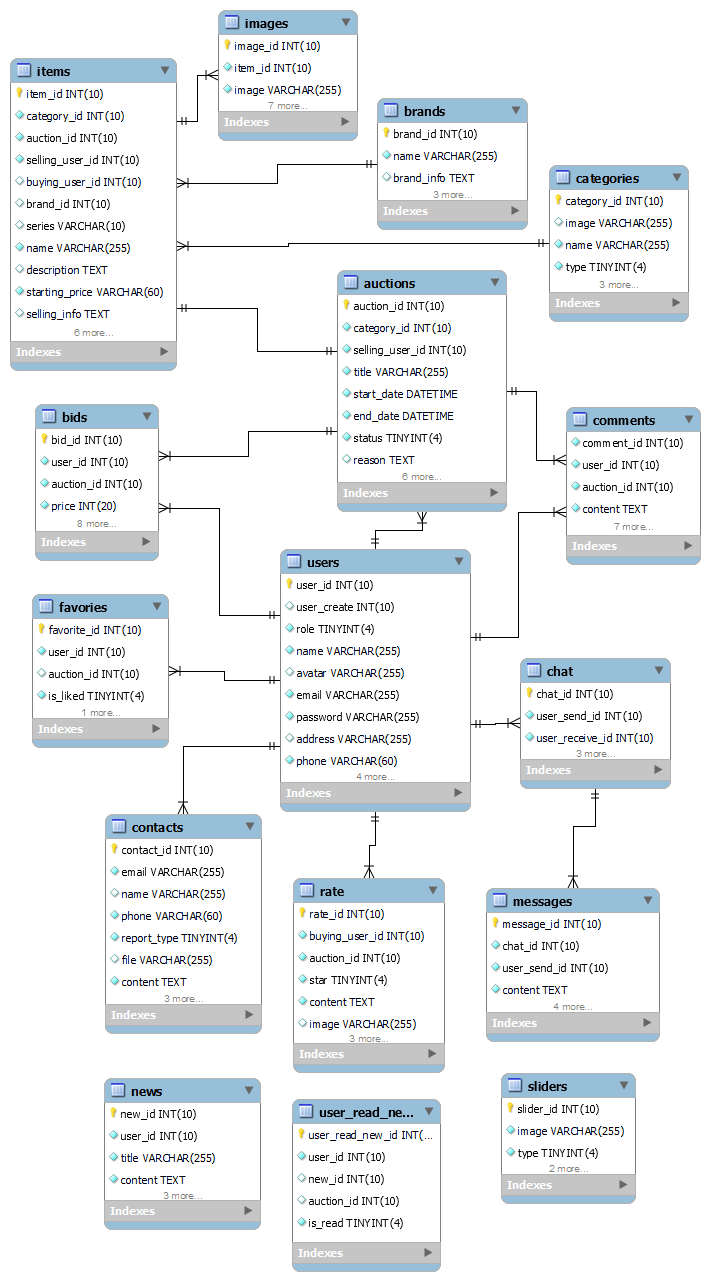
\includegraphics[width=0.75\linewidth,height=18cm]{Hinhve/err2.png}
    \caption{Sơ đồ thực thể liên kết}
    \label{fig:Fig413}
\end{figure}
Hình \ref{fig:Fig413} là sơ đồ thực thể liên kết cho cơ sở dữ liệu của hệ thống đấu giá trực tuyến. Ý nghĩa của từng thực thể được mô tả trong Bảng  \ref{bang48}
%\begin{table}[H]
    %\centering
    \tablehead{%
    \hline
    \bfseries Tên thực thể & \bfseries Ý nghĩa\\\hline}
    \tabletail{\hline}
    \topcaption{Ý nghĩa các thực thể}
    \label{bang48}
    \begin{supertabular}{| p{.30\textwidth} | p{.63\textwidth} |} 
    \hline
        auctions & Phiên đấu giá\\\hline
        users & Tài khoản người dùng\\\hline
        comments & Danh sách bình luận của phiên đấu giá\\\hline
        bids& Danh sách lượt trả giá của phiên đấu giá\\\hline
        items& Sản phẩm của phiên đấu giá\\\hline
        categories& Loại sản phẩm\\\hline
        brands& Thương hiệu sản phẩm\\\hline
        images& Danh sách hình ảnh của sản phẩm\\\hline
        favorites& Thích, không thích phiên đấu giá\\\hline
        contacts& Liên lạc với Quản trị viên\\\hline
        news& Tin tức\\\hline
        user\_read\_news& Tài khoản đã đọc tin tức chưa\\\hline
        chat& Danh sách cuộc nói chuyện\\\hline
        messages& Danh sách tin nhắn\\\hline
        rate& Danh sách đánh giá của phiên đấu giá\\\hline
        slides & Danh sách slide hiển thị trên trang chủ của người dùng\\\hline
    \end{supertabular}
%\end{table}
\section{Xây dựng ứng dụng}
\subsection{Thư viện và công cụ sử dụng}
%\begin{table}[H]
    %\centering
    \tablehead{%
    \hline
    \bfseries Mục đích & \bfseries Công cụ &\bfseries Địa chỉ URL\\\hline}
    \tabletail{\hline}
    \topcaption{Danh sách thư viện và công cụ sử dụng}
    \label{bang49}
    \begin{supertabular}{| p{.25\textwidth} | p{.25\textwidth} | p{.40\textwidth} |} 
    \hline
        IDE lập trình& Visual Studio Code& \href{https://code.visualstudio.com}{https://code.visualstudio.com} \\\hline
        Ngôn ngữ lập trình& Javascript& \href{https://www.javascript.com}{https://www.javascript.com} \\\hline
        Xây dựng giao diện& HTML& \href{https://developer.mozilla.org/en-US/docs/Web/HTML}{https://developer.mozilla.org/en-US/docs/Web/HTML} \\\hline
        Xây dựng giao diện& CSS& \href{https://developer.mozilla.org/en-US/docs/Web/CSS}{https://developer.mozilla.org/en-US/docs/Web/CSS} \\\hline
        Quản trị CSDL& MySQL& \href{https://www.mysql.com}{https://www.mysql.com} \\\hline
        Backend& PHP 7.1.32& \href{https://www.php.net}{https://www.php.net}\\\hline
        Backend Framework& Laravel 8& \href{https://laravel.com}{https://laravel.com} \\\hline
        Web UI Library& ReactJs 18.0.0& \href{https://reactjs.org/}{https://reactjs.org/}\\\cline{2-3}
                      & Material UI 5.6.1&\href{https://mui.com}{https://mui.com} \\\hline
        Phân tích thiết kế& Astah 8.5.0 & \href{https://astah.net/}{https://astah.net/} \\\cline{2-3}
                          & Diagram editor& \href{https://www.diagrameditor.com/}{https://www.diagrameditor.com/} \\\hline
    \end{supertabular}
%\end{table}
\subsection{Kết quả đạt được}
Từ những tìm hiểu và phân tích trên đồ án đã xây dựng Website đấu giá trực tuyến với các module chính: (i) Tìm kiếm, (ii) xem chi tiết phiên đấu giá, (iii) tạo phiên đấu giá, (iv) tham gia phiên đấu giá (trả giá, bình luận, đánh giá), (v) nhắn tin, (vi) yêu thích phiên đấu giá, (vii) xem tin tức, (viii) xem thông báo từ chối phiên đấu giá. Về hệ thống quản lý phía Quản trị viên là quản lý phê duyệt phiên đấu giá, quản lý việc thêm, sửa, xóa loại sản phẩm, thương hiệu, slide, tin tức.
%\begin{table}[H]
    %\centering
    \tablehead{%
    \hline
    \bfseries Thông tin & \bfseries Thống kê\\\hline}
    \tabletail{\hline}
    \topcaption{Thống kê thông tin ứng dụng server phía Người dùng}
    \label{bang410}
    \begin{supertabular}{| p{.45\textwidth}| p{.45\textwidth} |} 
    \hline
        Số dòng code& 4933\\\hline
        Dung lượng mã nguồn&233KB \\\hline
        Môi trường lập trình&Dell Vostro \\\hline
        Công cụ kiểm thử & Postman\\\hline
        Số bảng trong cơ sở dữ liệu  &16 bảng \\\hline
    \end{supertabular}
%\end{table}
\\
%\begin{table}[H]
    %\centering
    \tablehead{%
    \hline
    \bfseries Thông tin & \bfseries Thống kê\\\hline}
    \tabletail{\hline}
    \topcaption{Thống kê thông tin ứng dụng web}
    \label{bang411}
    \begin{supertabular}{| p{.45\textwidth}| p{.45\textwidth} |} 
    \hline
        Số dòng code& 8265\\\hline
        Dung lượng mã nguồn&950KB \\\hline
        Môi trường lập trình&Dell Vostro \\\hline
        Công cụ kiểm thử & Chrome Browser, Microsoft Edge\\\hline
    \end{supertabular}
%\end{table}
\\
%\begin{table}[H]
    %\centering
    \tablehead{%
    \hline
    \bfseries Thông tin & \bfseries Thống kê\\\hline}
    \tabletail{\hline}
    \topcaption{Thống kê thông tin ứng dụng phía Quản trị viên}
    \label{bang412}
    \begin{supertabular}{| p{.45\textwidth}| p{.45\textwidth} |} 
    \hline
        Số dòng code& 5077\\\hline
        Dung lượng mã nguồn&295KB \\\hline
        Môi trường lập trình&Dell Vostro \\\hline
        Công cụ kiểm thử & Chrome Browser, Microsoft Edge\\\hline
    \end{supertabular}
%\end{table}
\subsection{Minh họa các chức năng chính}
\begin{figure}[H]
    \centering
    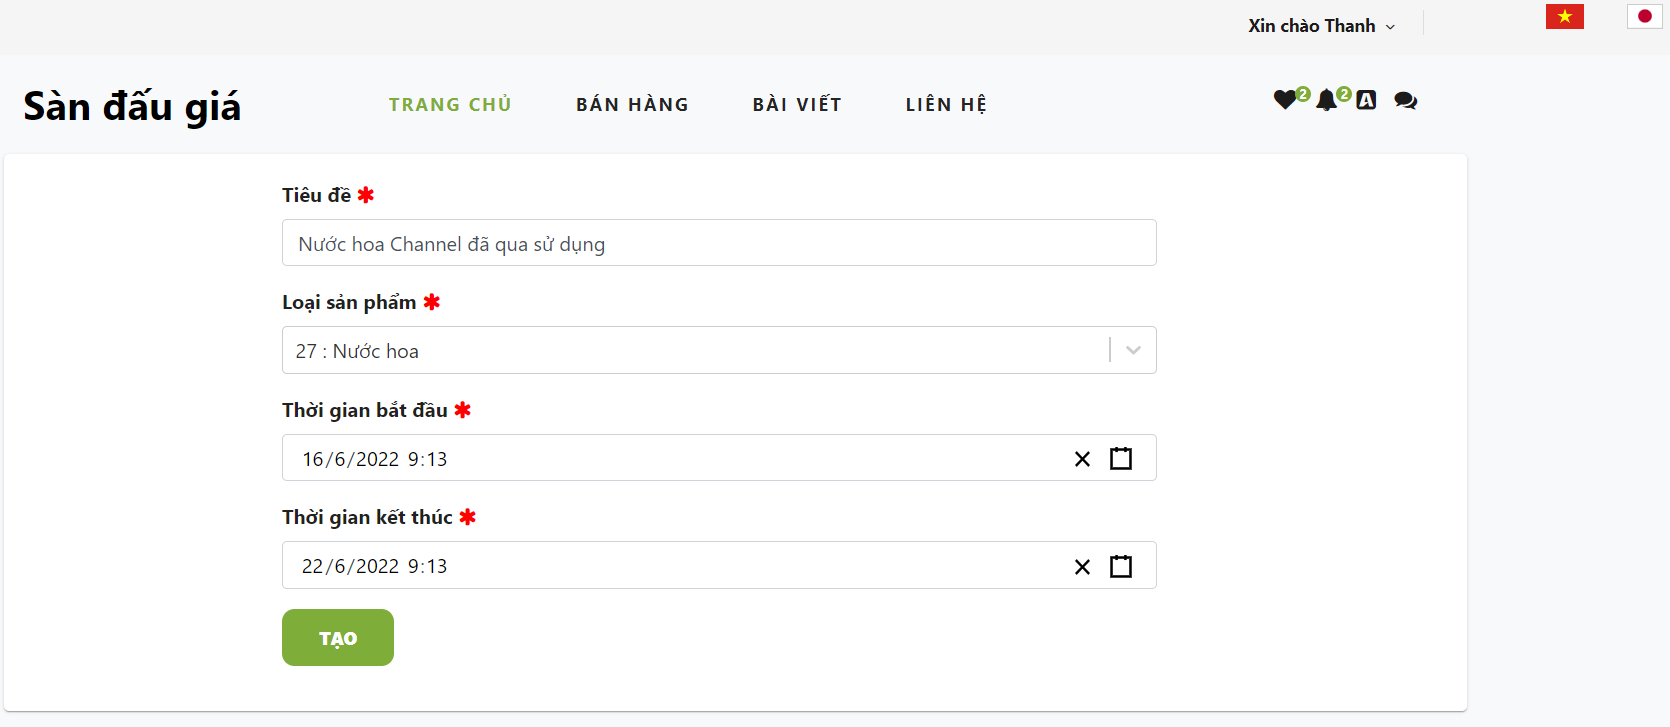
\includegraphics[width=0.75\linewidth,height=4.86cm]{Hinhve/createauctiondemo.png}
    \caption{Giao diện tạo phiên đấu giá}
    \label{fig:Fig414}
\end{figure}
Hình \ref{fig:Fig414} mô tả màn hình tạo phiên đấu giá. Người dùng đã có tài khoản thì có quyền được tạo phiên đấu giá. Người dùng điền thông tin phiên đấu giá vào form, đặc biệt với những trường nào có dấu sao màu đỏ là những trường bắt buộc phải nhập. Nếu người dùng không nhập hay nhập sai định dạng thông tin thì hệ thống sẽ báo lỗi tương ứng phía dưới ô đó. 
\begin{figure}[H]
    \centering
    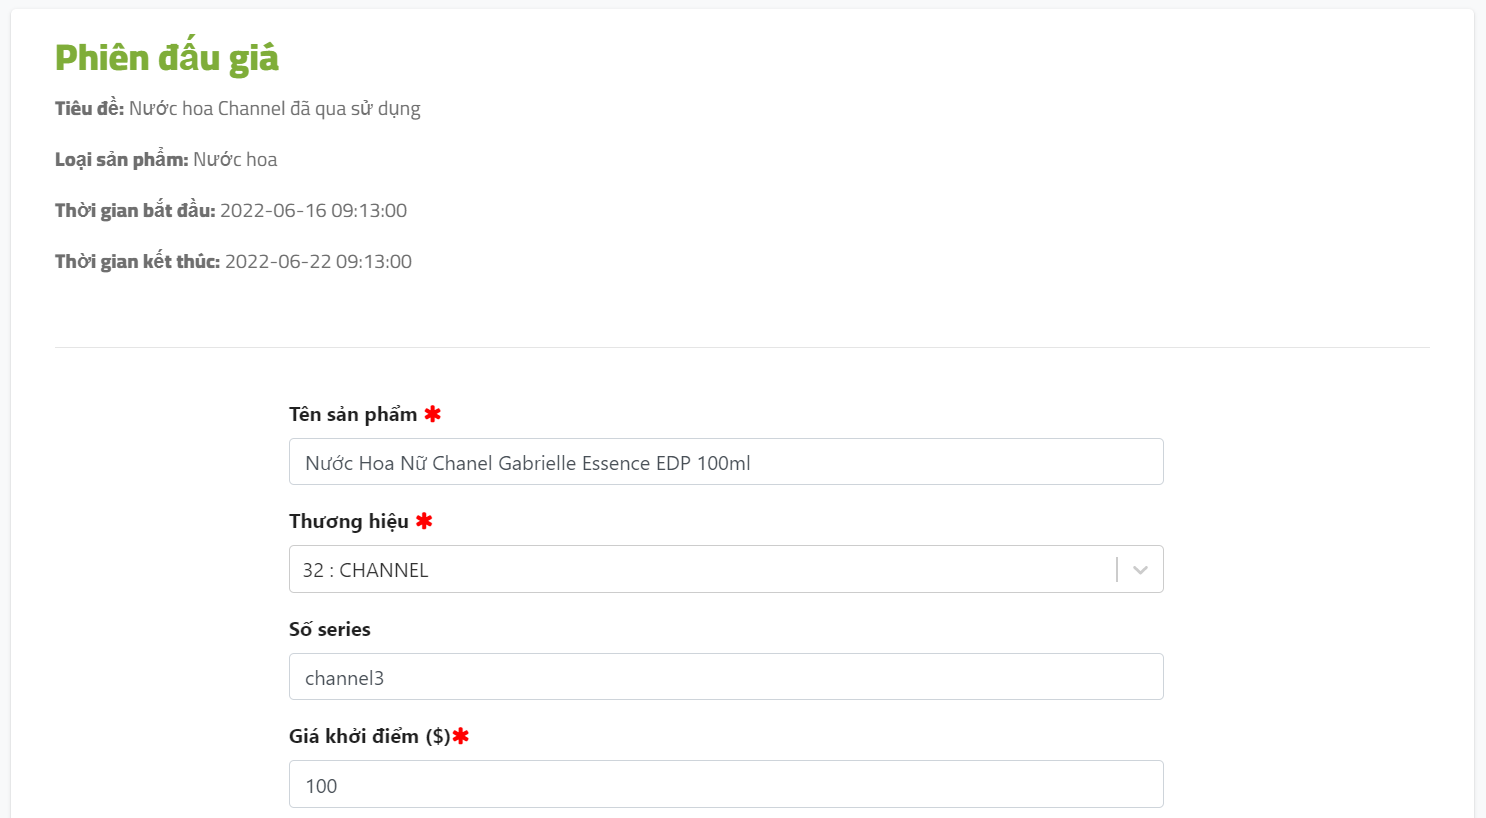
\includegraphics[width=0.75\linewidth,height=6.16cm]{Hinhve/createitem1demo.png}
    \label{fig:Fig4151}
\end{figure}
\begin{figure}[H]
    \centering
    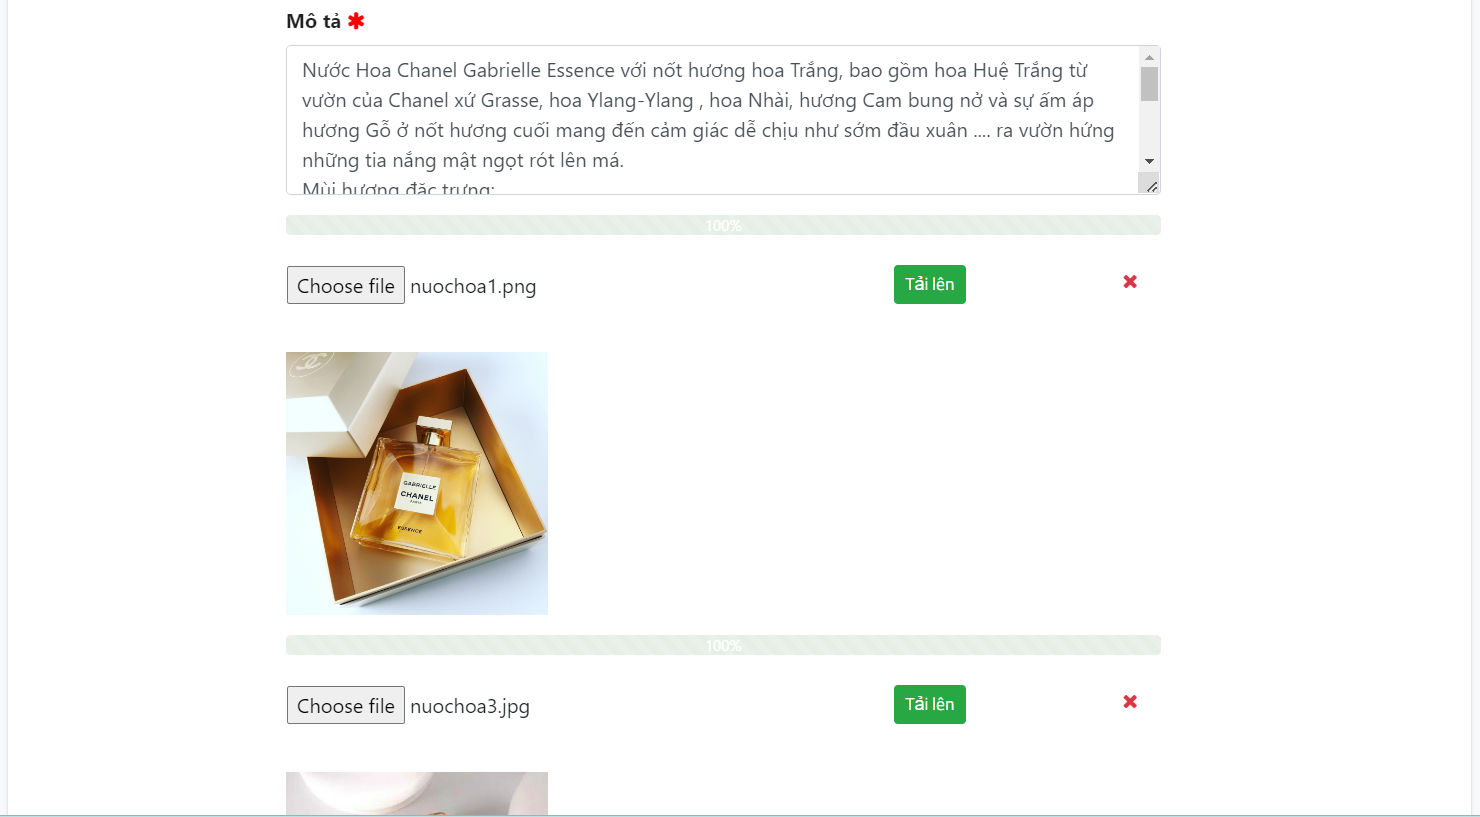
\includegraphics[width=0.75\linewidth,height=6.21cm]{Hinhve/createitem2demo.png}
    \caption{Giao diện tạo sản phẩm cho phiên đấu giá.}
    \label{fig:Fig415}
\end{figure}
Hình \ref{fig:Fig415} mô tả giao diện tạo sản phẩm cho phiên đấu giá. Người dùng sau khi tạo phiên đấu giá thì có thể thêm sản phẩm vào phiên đấu giá đó. Thông tin của phiên đấu giá được để lên đầu form tạo sản phẩm. Bên dưới là form tạo sản phẩm, người dùng nhập thông tin theo từng ô tương ứng. Nếu không nhập hay nhập sai thông tin thì hệ thống sẽ báo lỗi phía dưới trường đó.
\begin{figure}[H]
    \centering
    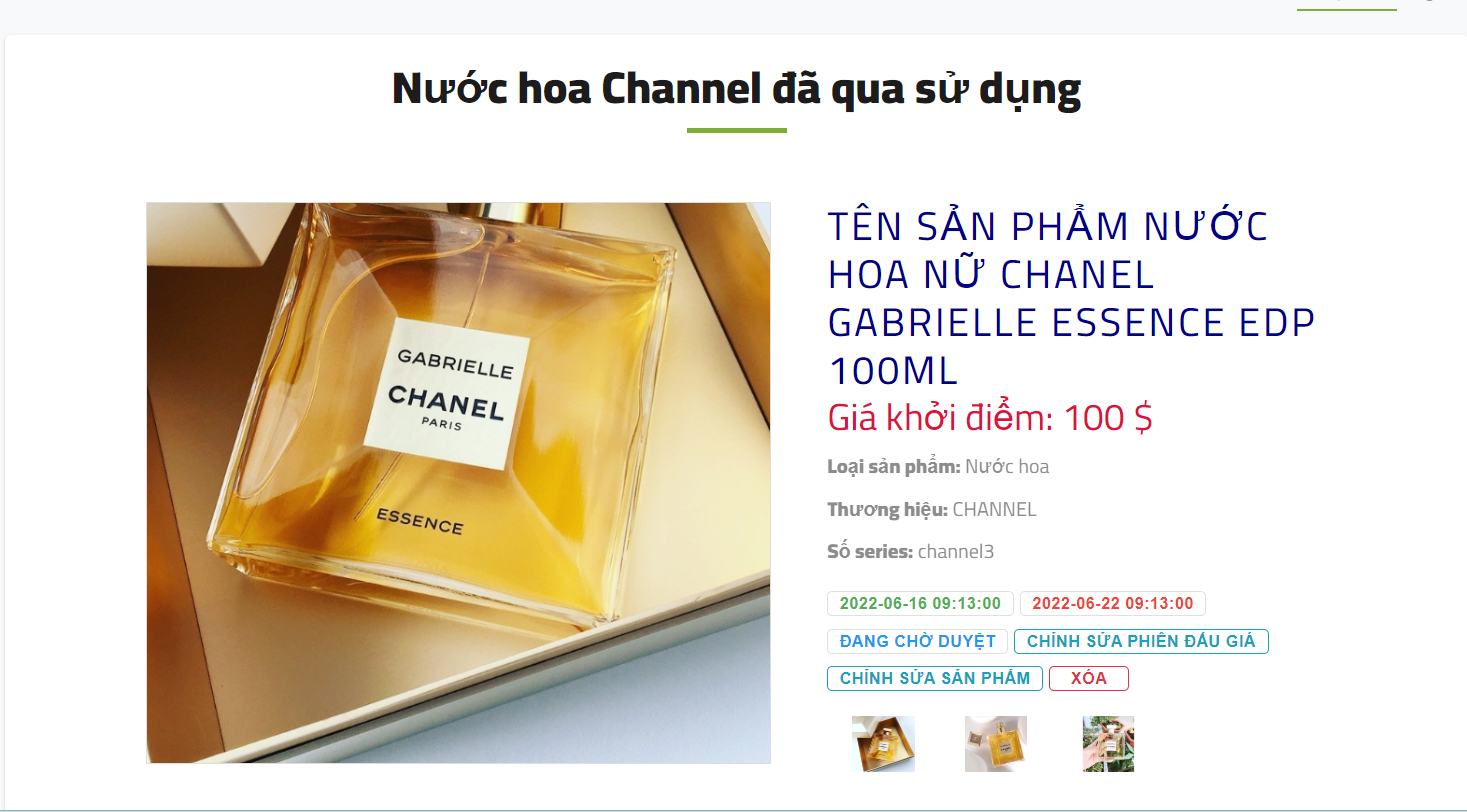
\includegraphics[width=0.75\linewidth,height=6.21cm]{Hinhve/auctionwait.png}
    \caption{Giao diện phiên đấu giá vừa tạo đang chờ duyệt.}
    \label{fig:Fig416}
\end{figure}
Hình \ref{fig:Fig416} mô tả giao diện phiên đấu giá vừa tạo đang chờ admin duyệt. Sau khi người dùng tạo phiên đấu giá và sản phẩm thì trong trang cá nhân của Người dùng sẽ hiển thị thông tin phiên đấu giá vừa tạo (bao gồm: tiêu đề phiên đấu giá đặt trên cùng, hình ảnh sản phẩm, sau đó là tên sản phẩm, giá khởi điểm, loại sản phẩm, thương hiệu, số series, label màu xanh thể hiện thời gian bắt đầu, màu đỏ thể hiện thời gian kết thúc và các button liên quan).\\
Trong trường hợp Người dùng tạo phiên đấu giá mà chưa thêm sản phẩm thì hệ thống hiển thị button Thêm sản phẩm, còn nếu đã Thêm sản phẩm rồi màn hình hiển thị các button chỉnh sửa, xóa phiên đấu giá đó. 
\begin{figure}[H]
    \centering
    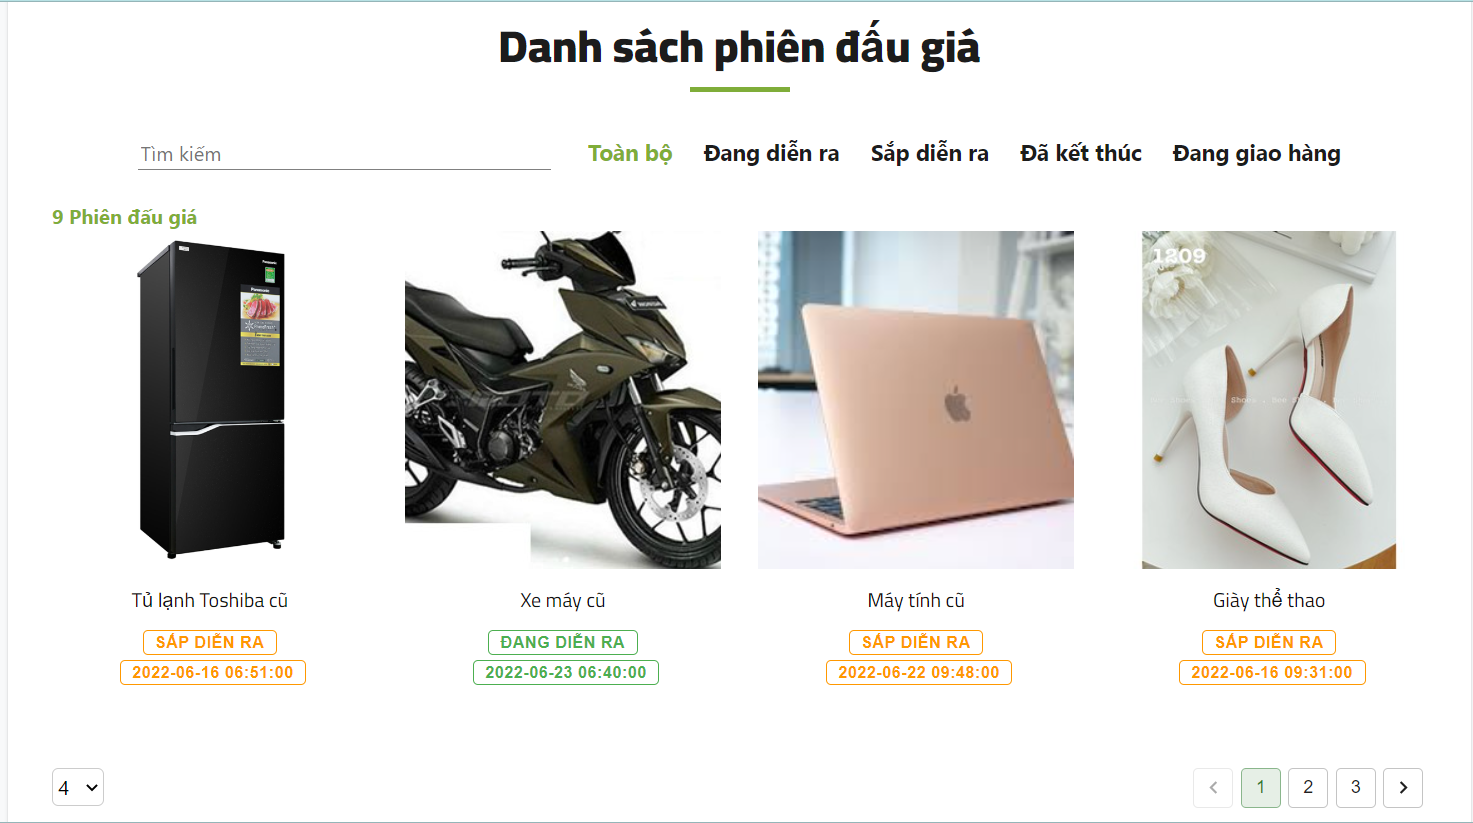
\includegraphics[width=0.75\linewidth,height=6.24cm]{Hinhve/listauctions.png}
    \caption{Giao diện danh sách phiên đấu giá toàn hệ thống}
    \label{fig:Fig417}
\end{figure}
Hình \ref{fig:Fig417} mô tả giao diện danh sách phiên đấu giá trên toàn hệ thống. Màn hình hiển thị các trạng thái, tổng số phiên đấu giá ở trạng thái đó, tên của phiên đấu giá, thời gian bắt đầu, thời gian kết thúc. Với các phiên đấu giá đang diễn ra, đã kết thúc sẽ hiển thị thời gian kết thúc, còn riêng đối với phiên đấu giá sắp diễn ra thì hiển thị thời gian bắt đầu. Màu sắc của các label được hiển thị theo trạng thái của phiên đấu giá đó. Hình ảnh đại diện là hình ảnh của loại sản phẩm thuộc phiên đấu giá đó. Mỗi trang có thể chọn hiển thị 4, 8, 12, 24 phiên đấu giá. Tại đây cũng có thể tìm kiếm phiên đấu giá theo tên, ngày giờ. 
\begin{figure}[H]
    \centering
    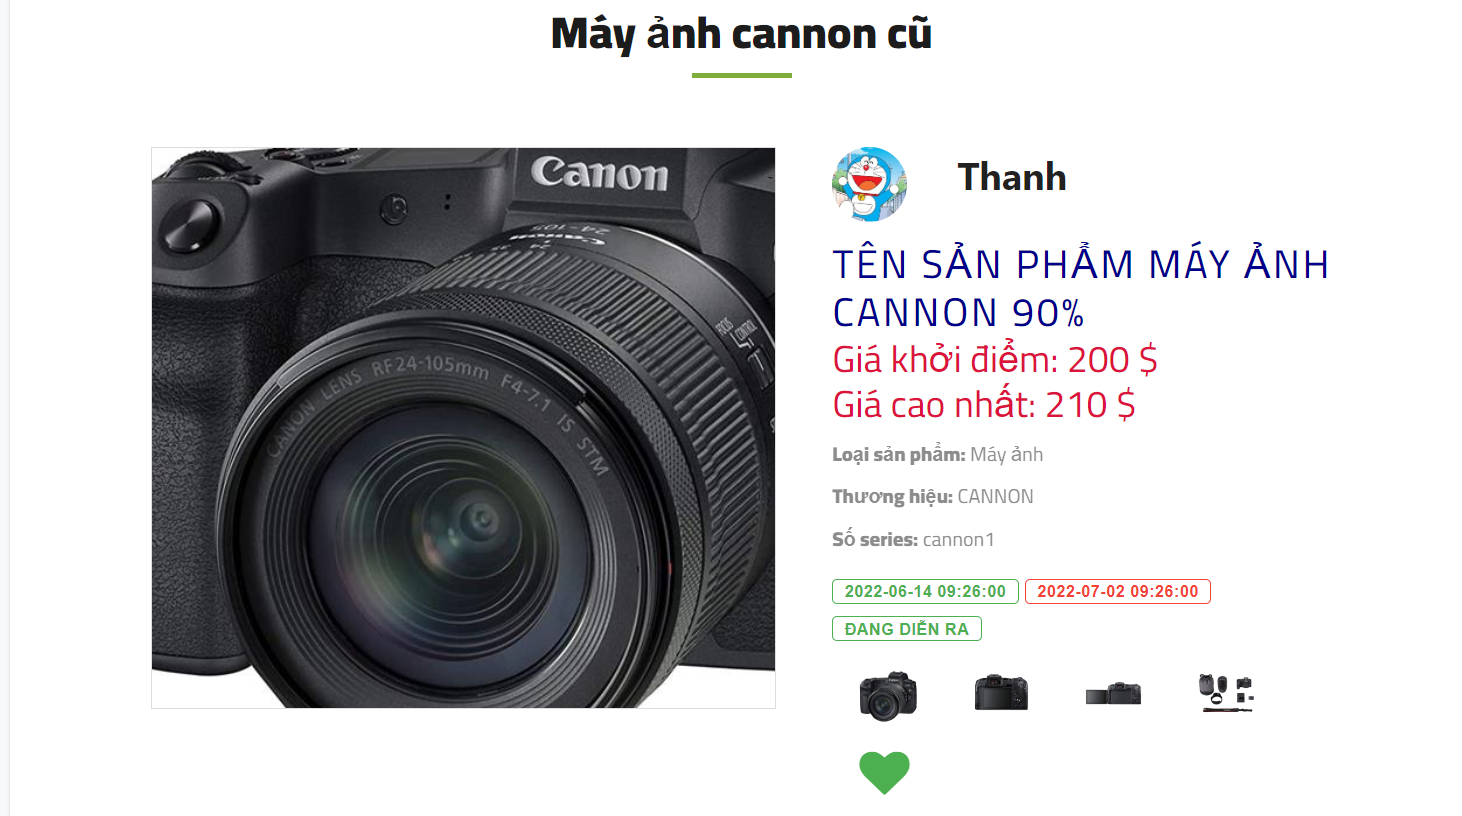
\includegraphics[width=0.75\linewidth,height=6.24cm]{Hinhve/auctionactive.png}
    \caption{Giao diện chi tiết phiên đấu giá đang diễn ra}
    \label{fig:Fig418}
\end{figure}
Hình \ref{fig:Fig418} mô tả giao diện chi tiết phiên đấu giá đang diễn ra. Giao diện này sẽ hiển thị tên phiên đấu giá ở trên cùng, tiếp đến là thông tin người bán, thông tin sản phẩm, trả giá cao nhất hiện tại, các hình ảnh của sản phẩm và icon trái tim để biết người dùng có yêu thích phiên đấu giá này không.
\begin{figure}[H]
    \centering
    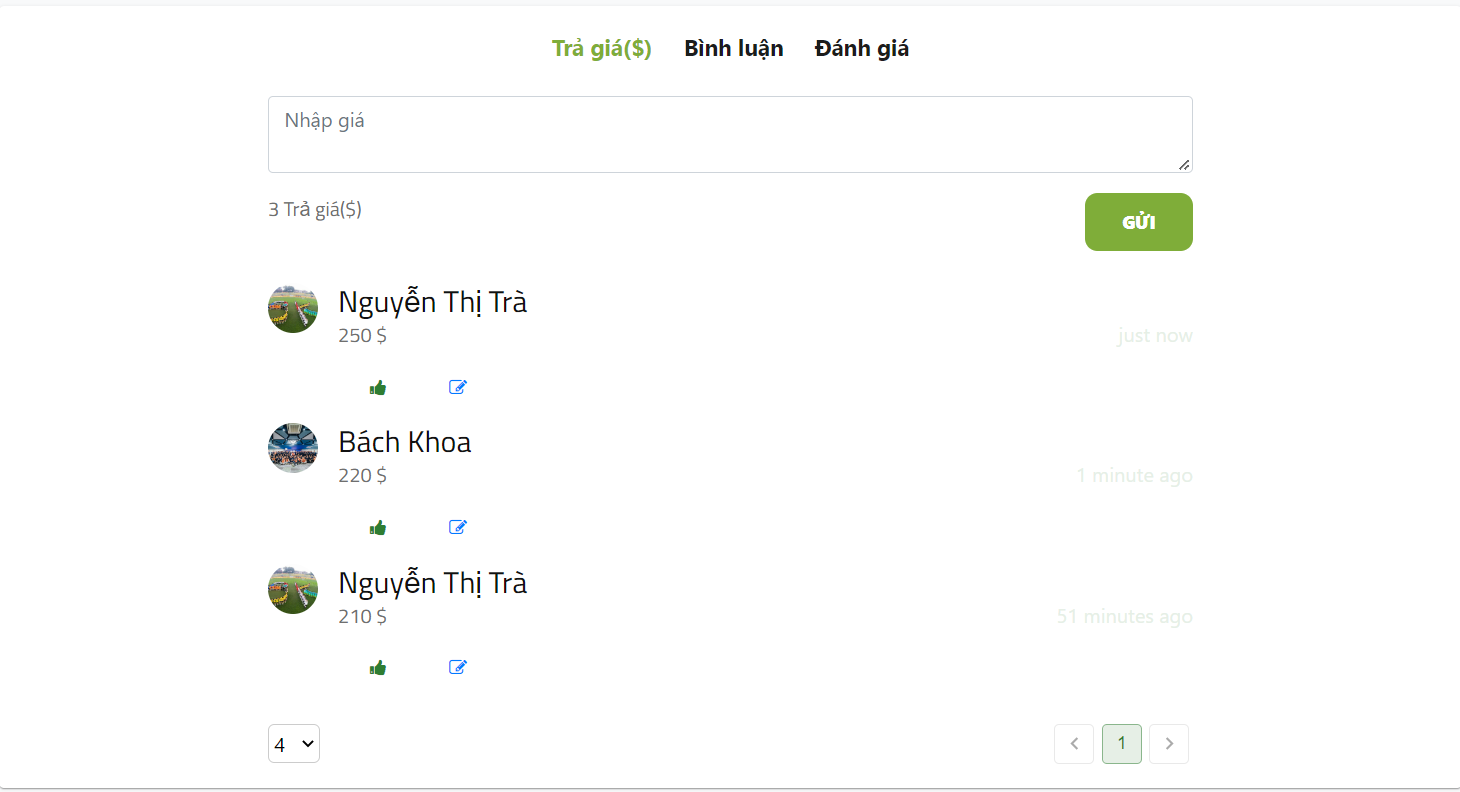
\includegraphics[width=0.75\linewidth,height=6.1cm]{Hinhve/commentbid.png}
    \caption{Giao diện các tab trả giá, bình luận, đánh giá của phiên đấu giá.}
    \label{fig:Fig419}
\end{figure}
Hình \ref{fig:Fig419} mô tả giao diện các tab trả giá, bình luận, đánh giá của phiên đánh giá. Giao diện này sẽ hiển thị người thực hiện hành động, nội dung hành động, thời gian tạo và tổng số lượt trả giá, bình luận hay đánh giá đang có của phiên đấu giá. 
\begin{figure}[H]
    \centering
    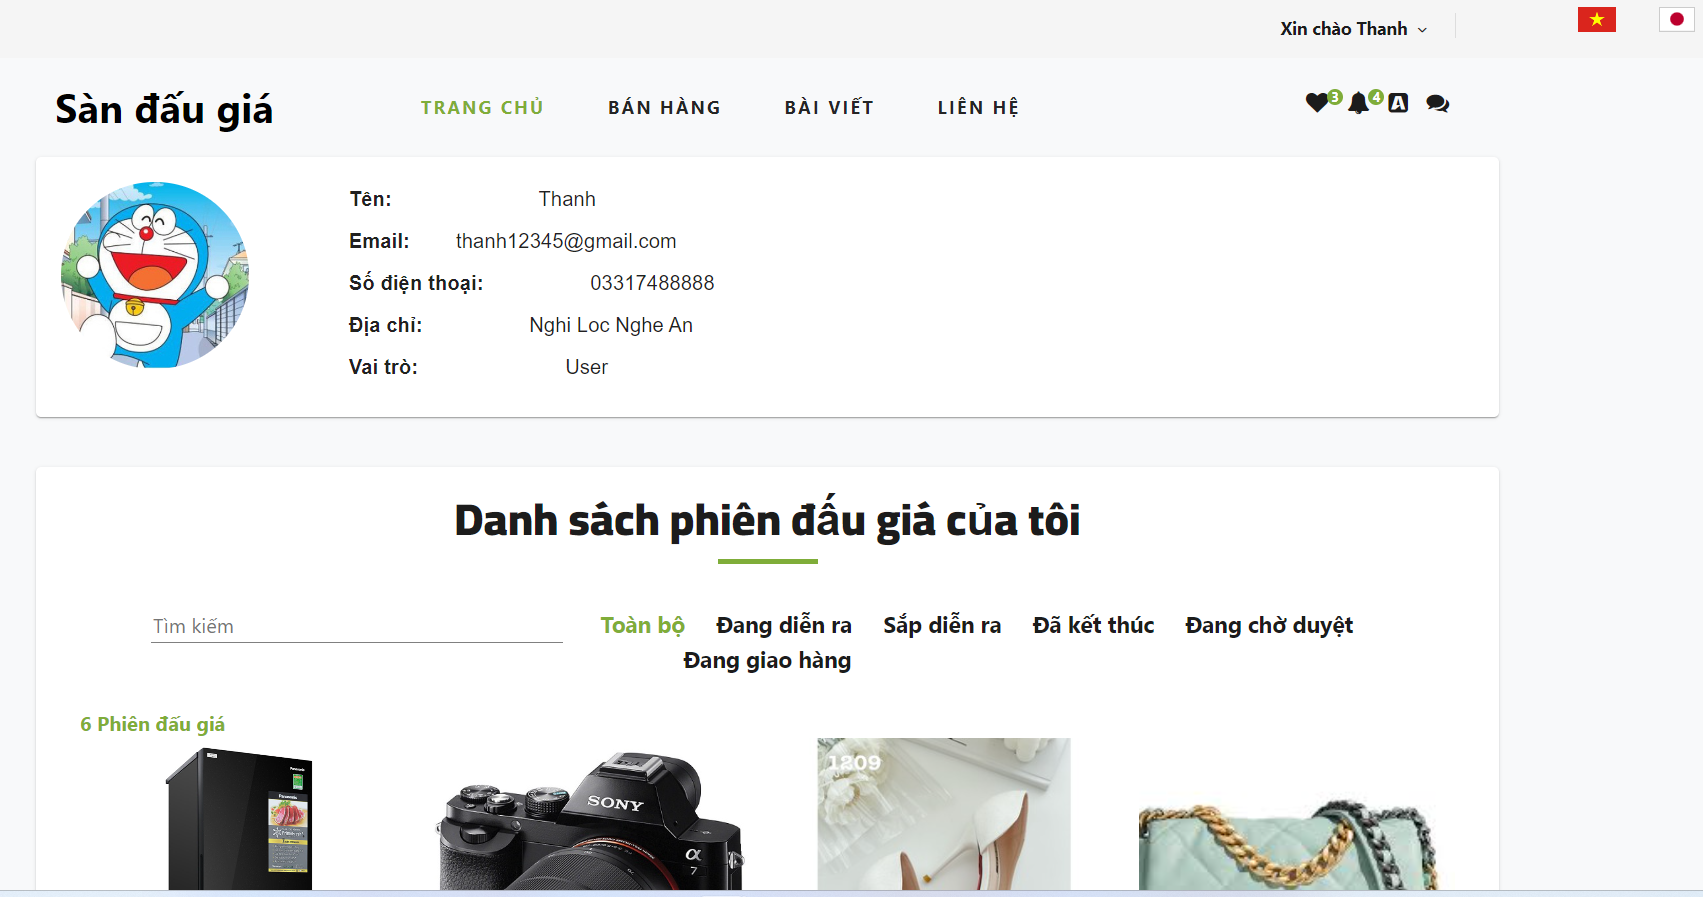
\includegraphics[width=0.75\linewidth,height=5.95cm]{Hinhve/vietnamese.png}
    \caption{Giao diện khi sử dụng ngôn ngữ là Tiếng Việt}
    \label{fig:Fig420}
\end{figure}
Hình \ref{fig:Fig420} mô tả giao diện khi sử dụng ngôn ngữ tiếng Việt. Khi người dùng chọn vào lá cờ Việt Nam thì ngôn ngữ trên hệ thống chuyển toàn bộ qua tiếng Việt. Tuy nhiên hiện tại hệ thống chỉ chuyển đổi những tiêu đề đã có sẵn trong hệ thống, còn thông tin người dùng nhập bằng ngôn ngữ nào thì vẫn giữ nguyên.
\begin{figure}[H]
    \centering
    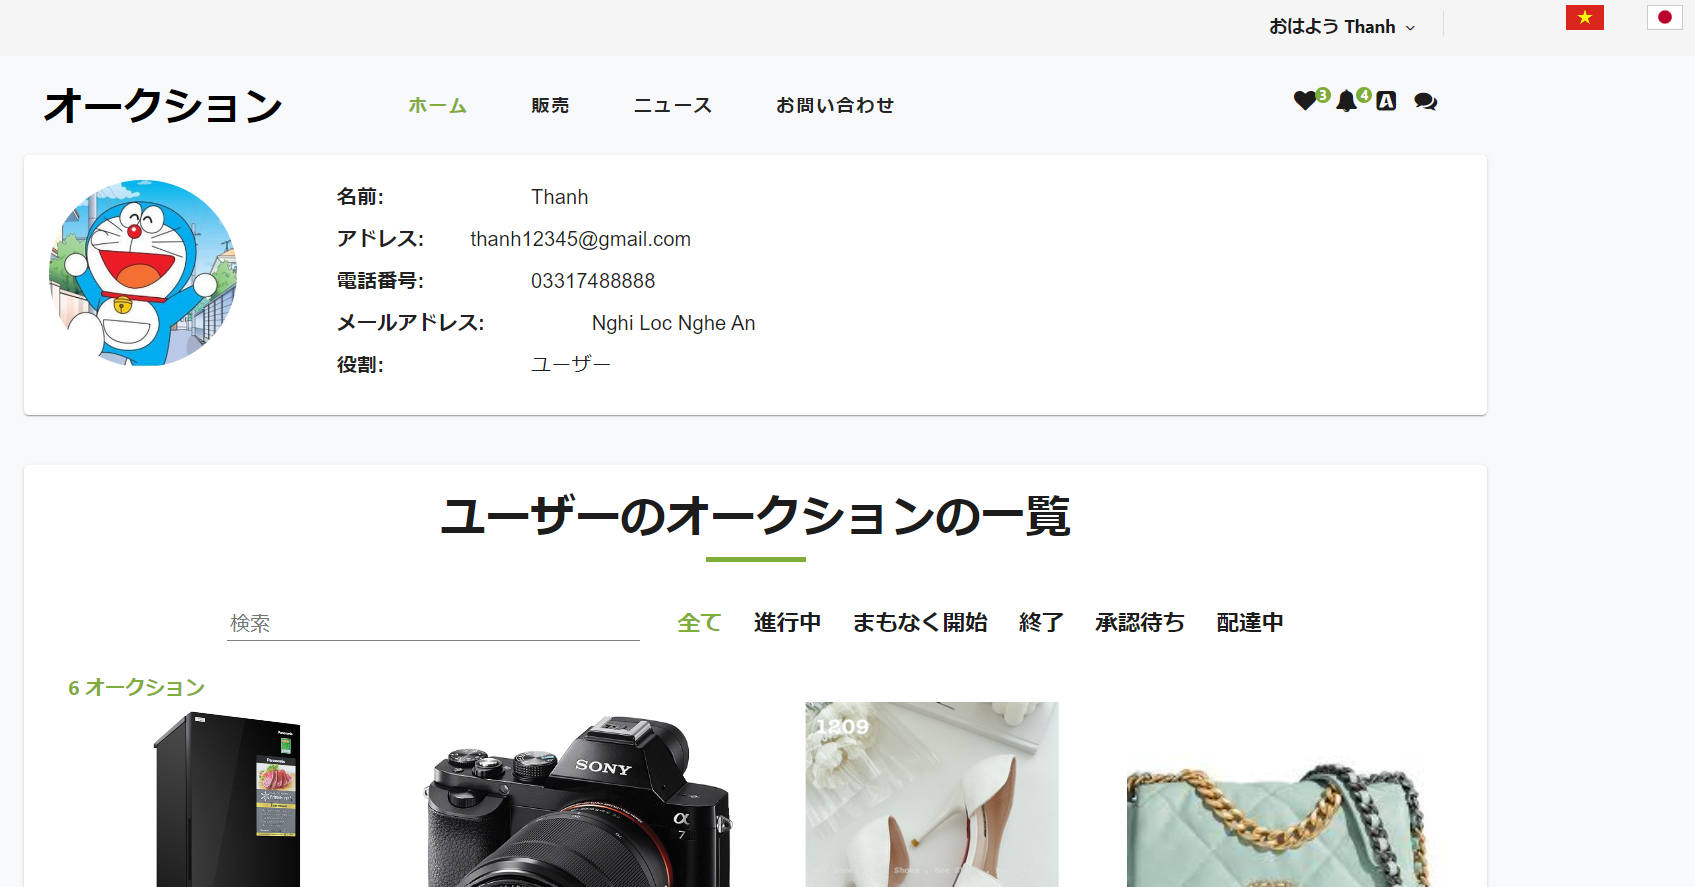
\includegraphics[width=0.75\linewidth,height=5.95cm]{Hinhve/jp.png}
    \caption{Giao diện khi chuyển ngôn ngữ qua tiếng Nhật}
    \label{fig:Fig421}
\end{figure}
Khi người dùng chọn vào lá cờ Nhật Bản thì ngôn ngữ trên hệ thống chuyển toàn bộ qua tiếng Nhật.
\section{Kiểm thử}
Để kiểm thử lại website đấu giá trực tuyến, sau khi kiểm thử API bằng Postman và ghép API hoàn chỉnh thì đồ án thực hiện bước kiểm thử sản phẩm sau cùng bằng kỹ thuật Black-Box trên môi trường Chrome browser, Microsoft Edge. Chi tiết kiểm thử một số chức năng được mô tả phía dưới. 
\subsection{Kiểm thử chức năng tạo phiên đấu giá}
%\begin{table}[H]
    %\centering
    \tablehead{%
    \hline
    \bfseries Đầu vào & \bfseries Đầu ra & \bfseries Kết quả\\\hline}
    \tabletail{\hline}
    \topcaption{Kiểm thử chức năng tạo phiên đấu giá}
    \label{bang413}
    \begin{supertabular}{| p{.45\textwidth}|p{.30\textwidth}|p{.15\textwidth}|} 
    \hline
        Bỏ trống “Tiêu đề”;
        Không chọn “Loại sản phẩm”;
        Không chọn “Thời gian bắt đầu”;
        Không chọn  “Thời gian kết thúc”.
        & Thông báo lỗi “Yêu cầu nhập” ở dưới trường bị bỏ trống&Đạt \\\hline
        Nhập “Tiêu đề” quá 255 ký tự
        & Thông báo lỗi “Tối đa 255 ký tự “&Đạt \\\hline
        Nhập “Thời gian bắt đầu” trước thời điểm hiện tại của ngày hôm sau.
        & Thông báo lỗi “ Thời gian bắt đầu sớm nhất từ ngày mai”&Đạt \\\hline
        Nhập “Thời gian kết thúc” sớm hơn “Thời gian bắt đầu”
        & Thông báo lỗi “Thời gian kết thúc phải sau Thời gian bắt đầu”&Đạt \\\hline
        Nhập “Thời gian bắt đầu” và “Thời gian kết thúc” không đúng định dạng ngày tháng
        & Thông báo lỗi “Không đúng định dạng”&Đạt \\\hline
    \end{supertabular}
%\end{table}
\subsection{Kiểm thử chức năng tạo sản phẩm cho phiên đấu giá}
%\begin{table}[H]
    %\centering
    \tablehead{%
    \hline
    \bfseries Đầu vào & \bfseries Đầu ra & \bfseries Kết quả\\\hline}
    \tabletail{\hline}
    \topcaption{Kiểm thử chức năng tạo sản phẩm cho phiên đấu giá}
    \label{bang414}
    \begin{supertabular}{| p{.45\textwidth}|p{.30\textwidth}|p{.15\textwidth}|} 
    \hline
        Bỏ trống “Tên sản phẩm”;
        Không chọn “Thương hiệu”;
        Bỏ trống “Giá khởi điểm”;
        Bỏ trống “Mô tả”.
        & Thông báo lỗi “Yêu cầu nhập” ở dưới trường bị bỏ trống&Đạt \\\hline
        Nhập “Tên sản phẩm” quá 255 ký tự
        & Thông báo lỗi “Tối đa 255 ký tự “&Đạt \\\hline
        Nhập “Số series” quá 10 ký tự
        & Thông báo lỗi “Tối đa 10 ký tự”&Đạt \\\hline
        Nhập “Giá khởi điểm” không đúng định dạng số
        & Thông báo lỗi “Hãy nhập số”&Đạt \\\hline
    \end{supertabular}
%\end{table}
\subsection{Kiểm thử chức năng phê duyệt phiên đấu giá}
%\begin{table}[H]
    %\centering
    \tablehead{%
    \hline
    \bfseries Đầu vào & \bfseries Đầu ra & \bfseries Kết quả\\\hline}
    \tabletail{\hline}
    \topcaption{Kiểm thử chức năng phê duyệt phiên đấu giá}
    \label{bang415}
    \begin{supertabular}{| p{.45\textwidth}|p{.30\textwidth}|p{.15\textwidth}|} 
    \hline
        Quản trị viên từ chối phiên đấu giá, khi nhập lý do từ chối thì bỏ trống trường “Lý do từ chối”.
        
        & Hiển thị toast cảnh báo “Bạn phải nhập lý do từ chối”.&Đạt \\\hline
        Sau khi Quản trị viên từ chối phiên đấu giá thì có thông báo đến cho người tạo phiên đấu giá không.
        & Hiển thị thông báo với tiêu đề lý do từ chối phiên đấu giá cho người tạo phiên đấu giá. Cập nhật trạng thái phiên đấu giá, xóa khỏi hệ thống. &Đạt \\\hline
        Quản trị viên chấp nhận phiên đấu giá
        & Cập nhật trạng thái phiên đấu giá, hiển thị lên hệ thống cho tất cả thành viên đều có thể xem được. &Đạt \\\hline
        Phiên đấu giá quá thời gian diễn ra mà vẫn không được phê duyệt
        & Hệ thống tự động cập nhật từ chối phiên đấu giá với lý do là “Quá thời gian duyệt”, gửi cho người tạo phiên đấu giá&Đạt \\\hline
    \end{supertabular}
%\end{table}
\section{Triển khai}
%\begin{table}[H]
    %\centering
    \tablehead{%
    \hline
    \bfseries Loại thiết bị/công cụ & \bfseries Yêu cầu\\\hline}
    \tabletail{\hline}
    \topcaption{Danh sách thiết bị, công cụ triển khai hệ thống}
    \label{bang416}
    \begin{supertabular}{| p{.30\textwidth}|p{.62\textwidth}|} 
    \hline
        Hệ điều hành& Hệ điều hành mã nguồn mở Linux: Ubuntu 14.04 LTS trở lên\\\hline
        CPU& Bộ xử lý tối thiểu: 2 nhân 1.7 GHz\\\hline
        GPU& Không yêu cầu\\\hline
        Bộ nhớ trong& Ram tối thiểu 1GB \\\hline
        Ổ đĩa& Còn trống ít nhất 1.5GB lưu trữ phần mềm \\\hline
        Hệ quản trị cơ sở dữ liệu&Hệ quản trị cơ sở dữ liệu MySQL \\\hline
    \end{supertabular}\\
%\end{table}
\\
Hệ thống sàn đấu giá trực tuyến hiện tại đang được triển khai trên localhost. Các bước chạy thử nghiệm trên localhost được thực hiện như sau: 
\begin{itemize}
    \item Bước 1: Cài đặt Docker theo trang chủ Docker \href{https://www.docker.com}{https://www.docker.com}.
    \item Bước 2: Đặt folder source code của auction-admin và auction-app vào chung một thư mục. 
    \item Bước 3: Tại folder source code của auction-admin chạy lệnh docker-compose up -d để building ứng dụng trên localhost.
    \item Bước 4: Cài đặt phần mềm quản lý cơ sở dữ liệu MySQL Workbench
    \item Bước 5: Chạy lệnh docker-exec -it auction-admin sh, sau đó để chạy lệnh php artisan migrate để cài đặt cơ sở dữ liệu trên hệ thống. Cuối cùng chạy lệnh composer install để cài đặt các thư viện hỗ trợ ứng dụng. Đường dẫn của hệ thống Quản trị viên là http://admin.localhost:443
    \item Bước 6: Tại folder auction-app chạy lệnh docker-exec -it auction-app sh, sau đó chạy lệnh composer install tại đây để cài đặt các thư viện hỗ trợ. Đường dẫn của api phía client là http://localhost:8080/
    \item Bước 7: Tại folder source code FontEnd chạy lệnh composer install để cài đặt các thư viện hỗ trợ, sau đó chạy lệnh npm start để bắt đầu ứng dụng. Tại folder socket trong folder source code FontEnd chạy lệnh npm start để kết nối ứng dụng client và server phục vụ cho tính năng realtime khi nhắn tin.
\end{itemize}
\newpage

\end{document}
